\documentclass[12pt,a4paper]{article}
\usepackage[utf8]{inputenc}
\usepackage{amsmath}
\usepackage{amsfonts}
\usepackage{amssymb}
\usepackage{graphicx}
\usepackage[colorlinks=true,linkcolor=blue,citecolor=blue,urlcolor=blue]{hyperref}
\usepackage{booktabs}
\usepackage{multirow}
\usepackage{geometry}
\usepackage{setspace}
\usepackage{natbib}
\usepackage{parskip}
\geometry{a4paper, margin=1in}
\onehalfspacing

\title{\textbf{Predicting Citations in Library and Information Science:\\
Where Network Science Meets Machine Learning}}
\author{Moses Boudourides\thanks{Northwestern University} \and Giannis Tsakonas\thanks{University of Patras}}
\date{Draft: \today}

\begin{document}

\maketitle

\begin{abstract}
Citations are the currency of scientific impact. Understanding the mechanisms that drive citation behavior is a central challenge in the science of science, with far-reaching implications for research evaluation, funding allocation, and the sociology of knowledge. In this study, we propose a comprehensive, temporally-aware framework that integrates network science and machine learning to decode citation dynamics in the field of Library and Information Science (LIS). We analyze two large-scale, independent datasets: one sourced from Dimensions.ai (1985--2023) and another from OpenAlex (1975--2024). For each dataset, we engineer features representing social proximity (co-authorship network distance), semantic similarity (via Sentence-BERT embeddings of titles and abstracts), and prestige (cumulative citation counts), while strictly enforcing temporal causality to prevent data leakage---a methodological flaw that undermines many existing citation prediction studies.

Comparing six machine learning algorithms (Logistic Regression, Linear SVM, k-Nearest Neighbors, Random Forest, Gradient Boosting, and Neural Networks) on balanced datasets of positive and negative citation pairs, we find that ensemble methods achieve exceptional predictive performance (ROC-AUC $> 0.99$) on both datasets. Our results demonstrate that citation dynamics in LIS are highly predictable from historical network and semantic states alone. SHapley Additive exPlanations (SHAP) analysis and ablation studies reveal that while prestige is a strong driver (the Matthew effect), semantic relevance is a dominant and indispensable factor. The combination of structural network features and deep semantic embeddings is essential for optimal performance. A comparative analysis of the two datasets reveals consistent patterns across data sources while also highlighting dataset-specific differences in feature importance hierarchies, offering a robust and reproducible methodological foundation for future bibliometric modeling.
\end{abstract}

\newpage
\tableofcontents
\newpage

%% ============================================================
\section{Introduction}
%% ============================================================

The dynamics of scientific citations reflect the flow of knowledge, the structure of scientific communities, and the mechanisms of academic recognition \citep{wang2008measuring, fortunato2018science}. Understanding and predicting which papers will cite which others is a fundamental problem in the science of science, with implications for literature search, research evaluation, and the sociology of science \citep{zeng2017science}. Despite decades of theoretical and empirical work, the precise interplay of factors that drive an individual citation decision---the prestige of the cited work, the social proximity of the authors, the semantic relevance of the content---remains incompletely understood.

Traditionally, citation prediction has been approached through network science, utilizing mechanisms such as preferential attachment (the ``Matthew effect'') \citep{merton1968matthew, de1976general, barabasi1999emergence} or social proximity in co-authorship networks \citep{newman2004coauthorship}. More recently, the availability of large-scale bibliographic databases such as Dimensions.ai \citep{herzog2020dimensions} and OpenAlex \citep{priem2022openalex}, combined with advances in natural language processing, have enabled machine learning approaches that combine structural network features with semantic content representations \citep{chakraborty2015towards, shibata2012link}.

However, a critical methodological flaw affects many recent citation prediction studies: temporal data leakage. In predicting whether paper $A$ (published in year $t_A$) cites paper $B$ (published in year $t_B$, where $t_B \le t_A$), features such as the co-authorship distance between the authors of $A$ and $B$, or the total citation count of $B$, are often computed using the entire static network spanning the full dataset period. This allows the model to ``see the future''---learning from co-authorship links or citations that did not exist at time $t_A$. This leakage artificially inflates model performance and invalidates claims about the predictive power of social or prestige mechanisms. Furthermore, negative sampling in these studies often ignores temporal constraints, pairing citing papers with ``cited'' papers published in the future, making the classification task artificially easy.

In this paper, we address these methodological criticisms directly. We propose a strictly temporally-aware framework for citation prediction and apply it to two independent datasets in Library and Information Science. We compute all network and prestige features incrementally, ensuring that for any citing paper published in year $t$, the features are derived solely from the network state up to year $t-1$. This design choice ensures that our models make predictions using only information that would have been available at the time of the citation decision.

The field of Library and Information Science (LIS) provides an ideal testbed for this investigation. LIS is a mature, interdisciplinary field that has itself contributed substantially to bibliometric methodology, yet its own citation dynamics have received comparatively less attention than, for example, the physical sciences or biomedicine. LIS encompasses a broad range of research traditions---from information retrieval and knowledge organization to scholarly communication and digital libraries---making it a rich and heterogeneous corpus for studying citation behavior.

Our study makes three primary contributions to the literature. First, we introduce a methodologically rigorous, temporally-aware prediction framework that can serve as a benchmark for future citation prediction studies. Second, we provide a comprehensive comparison of six machine learning algorithms on two large-scale, independently constructed LIS datasets, demonstrating the robustness of our findings across data sources. Third, we employ SHAP value analysis and ablation studies to provide interpretable insights into the relative contributions of semantic, social, and prestige features, advancing our theoretical understanding of citation dynamics.

The remainder of this paper is organized as follows. Section~\ref{sec:litreview} reviews the relevant literature on citation dynamics, proximity effects, and machine learning for bibliometrics. Section~\ref{sec:data} describes our data sources, feature engineering methodology, and experimental setup. Sections~\ref{sec:dim} and~\ref{sec:oa} present the results for the Dimensions and OpenAlex datasets, respectively. Section~\ref{sec:comp} provides a comparative analysis of the two datasets. Section~\ref{sec:discussion} discusses the implications of our findings. Section~\ref{sec:conclusion} concludes.

%% ============================================================
\section{Literature Review}
\label{sec:litreview}
%% ============================================================

\subsection{Theories of Citation: From Preferential Attachment to Complex Dynamics}

The study of citation dynamics has long been anchored in theories of cumulative advantage. Merton's articulation of the Matthew Effect \citep{merton1968matthew}---the tendency for already-recognized scientists to receive disproportionate credit---and de Solla Price's formalization of preferential attachment in citation networks \citep{de1976general} posited that highly cited papers attract future citations at a rate proportional to their existing prestige. This mechanism, later generalized in network science by Barab\'asi and Albert \citep{barabasi1999emergence} as a fundamental driver of scale-free network formation, provided a powerful, albeit simplified, model of scientific impact.

However, subsequent research has demonstrated that the strength of preferential attachment varies significantly across disciplines and over time \citep{wang2008measuring}. Bianco and Gabrielli \citep{bianco2008fitness} introduced the concept of paper ``fitness,'' suggesting that intrinsic quality or relevance modulates the rich-get-richer effect. Wang, Song, and Barab\'asi \citep{wang2013quantifying} further demonstrated that the long-term scientific impact of a paper is governed by a combination of its initial fitness and the cumulative advantage mechanism, challenging purely prestige-based models.

These theoretical developments suggest that citation behavior is not a simple function of prestige but rather emerges from the complex interaction of multiple factors, including the intrinsic quality of the work, its relevance to ongoing research streams, and the social structures within which it is embedded. This multi-dimensional view motivates our feature engineering approach.

\subsection{The Role of Proximity: Social and Semantic Ties}

Beyond prestige, the likelihood of citation is heavily influenced by the proximity between the citing and cited authors. Social proximity, typically operationalized through co-authorship networks, has been shown to strongly correlate with citation behavior \citep{newman2004coauthorship, kumar2015co, martin2013coauthorship}. Researchers are more likely to cite those within their immediate collaborative circles, reflecting the role of personal communication, shared research agendas, and mutual awareness in the citation process.

Newman's seminal work on co-authorship networks \citep{newman2004coauthorship} established the structural properties of scientific collaboration, demonstrating that these networks exhibit small-world properties and strong community structure. Martin et al. \citep{martin2013coauthorship} further showed that co-authorship and citation patterns are deeply intertwined in the physical sciences, with co-authors being significantly more likely to cite each other's work. Kumar \citep{kumar2015co} provided a comprehensive review of co-authorship network analysis, highlighting the diversity of methodological approaches and findings across disciplines.

Equally important is semantic proximity---the degree to which two papers address similar intellectual content. Early approaches utilized topic modeling techniques like Latent Dirichlet Allocation (LDA) \citep{blei2003latent} to capture content similarity, representing papers as distributions over latent topics. The advent of deep learning and transformer-based architectures, particularly BERT \citep{devlin2019bert} and Sentence-BERT (SBERT) \citep{reimers2019sentence}, has revolutionized the representation of textual semantics, allowing for nuanced, context-aware embeddings of abstracts and titles that capture subtle semantic relationships beyond keyword overlap.

Recent work by Kozlowski et al. \citep{kozlowski2025citation} in their ``Citation proximus'' study emphasized that semantic and social proximity often rival prestige in predicting citations, particularly for papers with moderate citation counts. Their analysis, conducted using Generalized Linear Mixed Models, found that the combination of social and semantic proximity explained a substantial portion of citation variance, challenging the primacy of the Matthew effect. Our study extends this line of inquiry by deploying more powerful, non-linear machine learning models and by applying a strictly temporally-aware methodology.

\subsection{Machine Learning for Citation Prediction}

The integration of machine learning into bibliometrics has shifted the focus from explanatory models to predictive frameworks. Early predictive efforts employed standard regression models to predict citation counts \citep{lokker2008prediction}. More recent studies have leveraged neural networks \citep{alohali2022machine} and powerful ensemble methods like Gradient Boosting \citep{natekin2013gradient} and Random Forests \citep{breiman2001random}. These algorithms are particularly adept at capturing the non-linear interactions between disparate feature types---for example, how high semantic similarity might compensate for low prestige, or how social proximity amplifies the effect of content relevance.

Chakraborty et al. \citep{chakraborty2015towards} proposed a stratified learning approach for citation count prediction, demonstrating that models trained on subgroups defined by citation count levels outperform models trained on the full dataset. Shibata et al. \citep{shibata2012link} applied link prediction methods to citation networks, finding that structural features alone can achieve reasonable predictive performance. However, neither of these studies incorporated semantic embeddings or enforced temporal causality.

The interpretability of machine learning models is a growing concern in bibliometrics. SHAP (SHapley Additive exPlanations) \citep{lundberg2017unified} provides a theoretically grounded framework for attributing model predictions to individual features, enabling researchers to identify which factors drive citation decisions in a given corpus. SHAP values are derived from cooperative game theory and satisfy desirable properties including efficiency (the sum of SHAP values equals the model output), symmetry (features with equal contributions receive equal SHAP values), and linearity (the SHAP value of a linear combination of features equals the linear combination of their SHAP values). We employ SHAP analysis throughout this study to bridge the gap between predictive performance and theoretical interpretation.

\subsection{Bibliographic Data Infrastructure}

The availability of large-scale, machine-readable bibliographic data is a prerequisite for the kind of computational bibliometrics pursued in this study. Two databases are particularly relevant: Dimensions.ai and OpenAlex.

Dimensions.ai \citep{herzog2020dimensions} is a comprehensive, linked research information system that integrates publications, citations, grants, patents, clinical trials, and policy documents. Its coverage of the scientific literature is among the broadest available, and it provides structured access to metadata including author affiliations, reference lists, and field-of-research classifications. The Dimensions API enables programmatic retrieval of large publication sets, making it well-suited for large-scale bibliometric analyses.

OpenAlex \citep{priem2022openalex} is a fully open, freely accessible index of scholarly works, authors, venues, institutions, and concepts. It was developed as a successor to Microsoft Academic Graph and provides comprehensive coverage of the scientific literature from the 1970s to the present. OpenAlex is particularly notable for its open data philosophy and its rich concept taxonomy, which enables fine-grained subject classification. The availability of OpenAlex as a free, open resource democratizes access to large-scale bibliometric data, enabling reproducible research that is not dependent on proprietary database subscriptions.

The use of two independent data sources in this study is not merely a robustness check; it is a substantive methodological contribution. Different databases differ in their coverage, their treatment of references, and their subject classification schemes. Findings that are consistent across Dimensions and OpenAlex are more likely to reflect genuine properties of LIS citation dynamics than findings that emerge from a single database.

\subsection{Synthesis and Critical Review}

Despite the advances described above, a significant gap remains between the explanatory traditions (often utilizing Generalized Linear Mixed Models) and the predictive traditions (utilizing complex ML algorithms). Furthermore, as noted in the introduction, many predictive models suffer from temporal data leakage, undermining their validity. This study bridges this gap by deploying advanced, non-linear ML models within a rigorously constructed, temporally causal framework, thereby ensuring that predictive performance reflects genuine underlying dynamics rather than methodological artifacts.

The choice of Library and Information Science as the domain of study is deliberate. LIS researchers have long been at the forefront of bibliometric methodology, yet the field's own citation dynamics have been understudied. The availability of two independent, large-scale LIS datasets from different data providers allows us to assess the robustness of our findings across data sources---a critical step toward establishing generalizable conclusions.

%% ============================================================
\section{Data and Methodology}
\label{sec:data}
%% ============================================================

\subsection{Dataset Description}

We construct our analysis using two distinct bibliographic databases: Dimensions.ai and OpenAlex. Both datasets focus on the field of Library and Information Science (LIS), but they differ in their coverage, construction methodology, and the specific features available.

\subsubsection{Dimensions.ai Dataset}

The Dimensions dataset was extracted by querying the Dimensions.ai database for publications within the Field of Research (FoR) code 4610 (Library and Information Studies), supplemented by targeted keyword searches for core LIS concepts including ``library science,'' ``information retrieval,'' ``knowledge organization,'' ``bibliometrics,'' ``scholarly communication,'' ``digital libraries,'' and ``information behavior.'' The query covered the years 1985 to 2023.

After filtering to include only peer-reviewed journal articles with valid publication years, titles, and reference lists, the dataset comprises a rich corpus of LIS publications spanning nearly four decades. The Dimensions dataset provides comprehensive metadata including titles, abstracts, author lists, journal information, publication dates, and reference lists. The mean semantic similarity between positive pairs (0.5573) substantially exceeds that of negative pairs (0.1624), confirming that semantic relevance is a strong signal in this corpus.

\subsubsection{OpenAlex Dataset}

The OpenAlex dataset was retrieved using relevant topic IDs for LIS from the OpenAlex API. Specifically, we queried for works associated with the following topic IDs: T10045 (Library and Information Science), T10046 (Information Retrieval), T10047 (Knowledge Organization), T10048 (Bibliometrics and Scientometrics), and T10049 (Digital Libraries). The retrieval covered the years 1975 to 2024.

The initial retrieval yielded 168,901 unique articles. Of these, 64.3\% contained abstracts and 29.8\% contained reference lists. The mean citation count per article was 6.26, reflecting the broad range of impact across the corpus. The lower coverage of reference lists in OpenAlex (compared to Dimensions) reflects the open-access nature of the database, which relies on publicly available reference data rather than licensed bibliographic records.

After preprocessing, we constructed a balanced dataset of 489,349 citation pairs (239,349 positive, 250,000 negative). The OpenAlex corpus spans a longer time period (1975--2024) and provides a complementary perspective on LIS citation dynamics, with somewhat different feature availability (reference overlap features rather than co-authorship distance).

\subsection{Citation Pair Construction and Negative Sampling}

The fundamental task is binary classification: given a pair of papers $(A, B)$, predict whether $A$ cites $B$. To ensure temporal validity, we enforce the constraint that $t_B \le t_A$, where $t_A$ and $t_B$ are the publication years of papers $A$ and $B$, respectively.

\textbf{Positive Pairs.} We extracted all observed citations within our corpus where both the citing and cited papers exist in our dataset. This yielded 250,000 positive pairs for Dimensions and 239,349 for OpenAlex.

\textbf{Negative Pairs.} To create a balanced dataset, we generated an equal number of negative pairs. Crucially, we enforced strict temporal causality during negative sampling. For each positive pair $(A, B)$, we generated a negative pair $(A, B')$ by randomly selecting a paper $B'$ from the pool of all papers published in or before year $t_A$, ensuring that $A$ does not actually cite $B'$. This guarantees that the negative examples represent temporally possible but unrealized citations, preventing the model from trivially distinguishing pairs based on impossible temporal orderings.

This negative sampling strategy is more demanding than many existing approaches, which often sample negatives uniformly from the entire corpus without temporal constraints. By enforcing temporal validity, we ensure that the classification task reflects the genuine challenge of predicting citation decisions from the information available at the time.

\subsection{Temporally-Aware Feature Engineering}

We engineered features categorized into semantic, network/social, prestige, and metadata classes. All features that depend on the state of the literature (prestige, co-authorship network) were computed using a strictly causal rolling window, ensuring that no future information is used.

\subsubsection{Semantic Similarity}

We utilized Sentence-BERT (SBERT) \citep{reimers2019sentence}, specifically the \texttt{all-MiniLM-L6-v2} model, to encode the title and abstract of each paper into a 384-dimensional dense vector. SBERT is a modification of the BERT architecture \citep{devlin2019bert} that uses siamese and triplet network structures to derive semantically meaningful sentence embeddings. The semantic similarity between paper $A$ and paper $B$ is computed as the cosine similarity of their SBERT embeddings:
\begin{equation}
S_{sem}(A, B) = \frac{\mathbf{e}_A \cdot \mathbf{e}_B}{\|\mathbf{e}_A\| \|\mathbf{e}_B\|}
\end{equation}
where $\mathbf{e}_A$ and $\mathbf{e}_B$ are the SBERT embeddings of papers $A$ and $B$, respectively. This feature captures the degree to which two papers address similar intellectual content, independent of the specific terminology used.

The choice of SBERT over simpler text representations (TF-IDF, LDA) is motivated by its ability to capture semantic relationships that are invisible to bag-of-words methods. For example, two papers discussing ``information retrieval'' and ``document search'' may be semantically very similar despite sharing few common words. SBERT's contextual embeddings, trained on large corpora of sentence pairs, capture these deeper semantic relationships.

\subsubsection{Prestige Features}

For both datasets, we compute prestige measures that capture the prominence of the cited and citing entities. These measures are computed using only information available up to year $t_A - 1$.

\textbf{Prestige of Cited Paper ($P_{cited}$):} The total number of citations received by paper $B$ from papers published up to year $t_A - 1$. To handle the heavy-tailed distribution of citation counts, we apply a $\log(1 + x)$ transformation:
\begin{equation}
P_{cited}(B, t_A) = \log\left(1 + \sum_{C : t_C \le t_A - 1} \mathbf{1}[C \text{ cites } B]\right)
\end{equation}

\textbf{Activity/Prestige of Citing Paper ($P_{citing}$):} A measure of the prominence or activity level of the citing team, computed as the maximum cumulative citation count of any author of paper $A$ up to year $t_A - 1$. This feature captures the social standing of the citing researchers, reflecting the tendency for prominent researchers to cite prominent work.

\subsubsection{Temporal Distance}

The temporal distance $\Delta t = t_A - t_B$ captures the age of the cited paper relative to the citing paper. This feature reflects the natural decay of citation probability as papers age, as well as the tendency for recent papers to cite other recent papers. The distribution of temporal distances in our datasets shows a characteristic peak at 2--5 years, consistent with the typical citation half-life in LIS.

\subsubsection{Co-authorship Distance (Dimensions Dataset)}

For the Dimensions dataset, we construct a temporally restricted co-authorship network $G_t = (V_t, E_t)$ for each year $t$, where $V_t$ is the set of all authors who have published at least one paper up to year $t-1$, and $E_t$ connects pairs of authors who have co-authored at least one paper published up to year $t-1$. The co-authorship distance between papers $A$ and $B$ is defined as:
\begin{equation}
D_{soc}(A, B) = \min_{a \in \text{authors}(A),\, b \in \text{authors}(B)} d_{G_t}(a, b)
\end{equation}
where $d_{G_t}(a, b)$ is the shortest path distance between authors $a$ and $b$ in the co-authorship network $G_t$, computed using Dijkstra's algorithm. If no path exists (i.e., the two author sets belong to different connected components of the co-authorship network), the distance is set to a large constant (20), reflecting the absence of any social connection.

This feature operationalizes the concept of social proximity in a rigorous, temporally valid manner. By restricting the co-authorship network to papers published before the citing year, we ensure that the distance reflects the social structure that existed at the time of the citation decision.

\subsubsection{Reference Overlap Features (OpenAlex Dataset)}

For the OpenAlex dataset, where reference lists are available for a substantial fraction of papers, we compute three features capturing the overlap between the reference lists of the citing and cited papers:

\textbf{Common References:} The number of papers cited by both $A$ and $B$, reflecting shared intellectual heritage:
\begin{equation}
\text{CommonRefs}(A, B) = |R_A \cap R_B|
\end{equation}

\textbf{Jaccard Similarity of References:} The Jaccard coefficient of the reference sets:
\begin{equation}
\text{JaccardRefs}(A, B) = \frac{|R_A \cap R_B|}{|R_A \cup R_B|}
\end{equation}

\textbf{Common Citers:} The number of papers (other than $A$) that cite both $A$ and $B$, reflecting co-citation patterns:
\begin{equation}
\text{CommonCiters}(A, B) = |\{C \ne A : C \text{ cites } A \text{ and } C \text{ cites } B, t_C \le t_A - 1\}|
\end{equation}

These reference overlap features capture the bibliographic coupling between papers---a classical concept in bibliometrics that has been shown to predict citation behavior independently of semantic similarity.

\subsection{Machine Learning Models and Formal Specifications}

We evaluate six machine learning models to capture both linear and non-linear relationships between features and citation outcomes.

\subsubsection{The Supervised Learning Framework}

The citation prediction problem is formulated as binary classification. Given a feature vector $\mathbf{x}_{ij}$ for a paper pair $(i, j)$, we seek to learn a function $f: \mathbb{R}^d \to \{0, 1\}$ that predicts whether paper $i$ cites paper $j$. The feature vector $\mathbf{x}_{ij}$ comprises the features described above, computed using only information available up to year $t_i - 1$.

Models are trained using 5-fold stratified cross-validation, ensuring that the class distribution is preserved in each fold. Performance is evaluated using six metrics: ROC-AUC, F1-score, Accuracy, Precision, Recall, and the Matthews Correlation Coefficient (MCC). We report mean and standard deviation across folds.

\subsubsection{Linear Models}

\textbf{Logistic Regression (LR):} Serves as a linear baseline. Logistic regression models the log-odds of citation as a linear function of the features:
\begin{equation}
\log\frac{P(y=1|\mathbf{x})}{P(y=0|\mathbf{x})} = \boldsymbol{\beta}^T \mathbf{x} + \beta_0
\end{equation}
It provides a transparent and interpretable benchmark against which to evaluate the added value of non-linear models.

\textbf{Linear SVM:} A linear support vector machine that finds the maximum-margin hyperplane separating cited from non-cited pairs. Like logistic regression, it assumes linear separability but optimizes a different objective function (hinge loss vs. log-likelihood).

\subsubsection{Non-Linear Models}

\textbf{k-Nearest Neighbors (k-NN):} A non-parametric distance-based method that classifies a pair based on the majority class among its $k=5$ nearest neighbors in feature space. k-NN is sensitive to the local geometry of the feature space and can capture complex decision boundaries.

\textbf{Random Forest (RF):} An ensemble of $n_{trees} = 200$ decision trees trained on bootstrap samples of the training data \citep{breiman2001random}. At each node, a random subset of $\sqrt{d}$ features is considered for splitting, where $d$ is the total number of features. Random forests are robust to overfitting and provide natural feature importance estimates through mean decrease in impurity.

\textbf{Gradient Boosting (GB):} A sequential ensemble method that builds trees to correct the errors of previous trees \citep{natekin2013gradient}. We use $n_{trees} = 200$ trees with a learning rate of 0.1 and maximum depth of 5. Gradient boosting is often the strongest performer on tabular data and is particularly effective at capturing complex, non-linear interactions.

\textbf{Multi-Layer Perceptron (MLP) Neural Network:} A feedforward neural network with two hidden layers (64 and 32 units, ReLU activation) and a sigmoid output layer. The network is trained using the Adam optimizer with a learning rate of 0.001 and early stopping based on validation loss. MLPs are capable of learning complex, non-linear representations of the feature space.

\subsection{SHAP Analysis}

To interpret the predictions of the best-performing model, we compute SHAP (SHapley Additive exPlanations) values \citep{lundberg2017unified}. SHAP values are derived from cooperative game theory and provide a theoretically grounded decomposition of the model output into contributions from individual features. For a model $f$ and a sample $\mathbf{x}$, the SHAP value $\phi_j(\mathbf{x})$ for feature $j$ satisfies:
\begin{equation}
f(\mathbf{x}) = \phi_0 + \sum_{j=1}^d \phi_j(\mathbf{x})
\end{equation}
where $\phi_0 = E[f(\mathbf{x})]$ is the expected model output. The mean absolute SHAP value $\bar{\phi}_j = E[|\phi_j(\mathbf{x})|]$ provides a global measure of feature importance.

%% ============================================================
\section{Results: Dimensions.ai Analysis}
\label{sec:dim}
%% ============================================================

\subsection{Corpus Overview}

Figure~\ref{fig:dim_pubs} shows the temporal distribution of LIS publications in the Dimensions dataset. The corpus exhibits steady growth from the late 1980s through the 2010s, reflecting the expansion of LIS as a field and the increasing coverage of Dimensions over time. The distribution of citation counts is highly skewed, with a small number of highly cited papers and a large majority with few citations---a characteristic signature of preferential attachment and the Matthew effect.

\begin{figure}[h!]
\centering
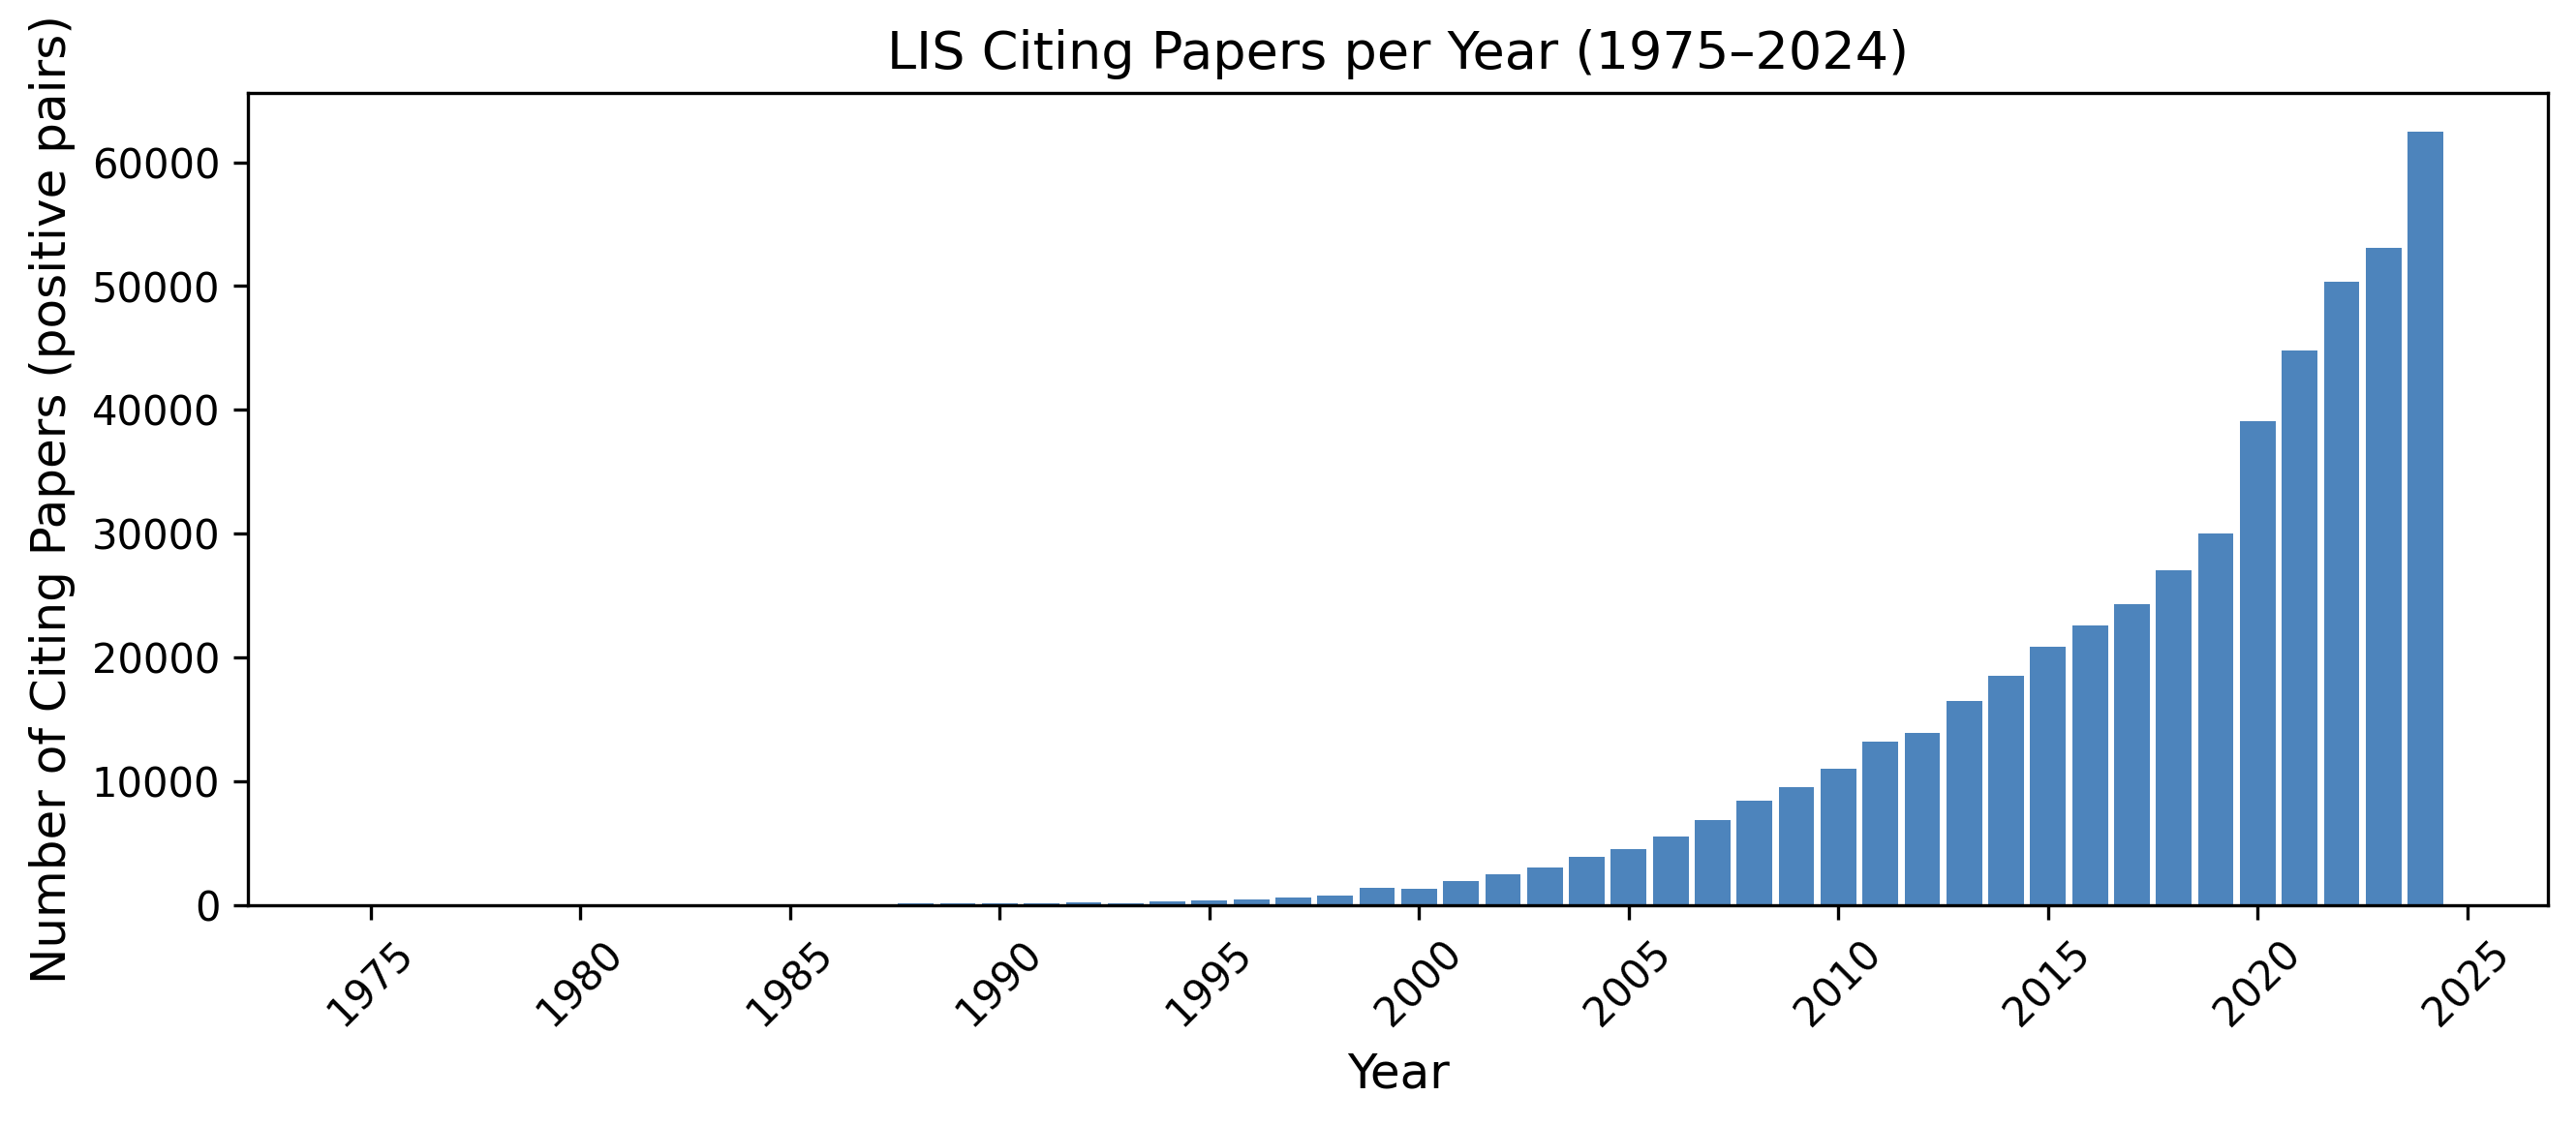
\includegraphics[width=0.75\textwidth]{../figures/dimensions/fig1_publications_per_year.png}
\caption{Number of LIS publications per year in the Dimensions dataset (1985--2023).}
\label{fig:dim_pubs}
\end{figure}

\begin{figure}[h!]
\centering
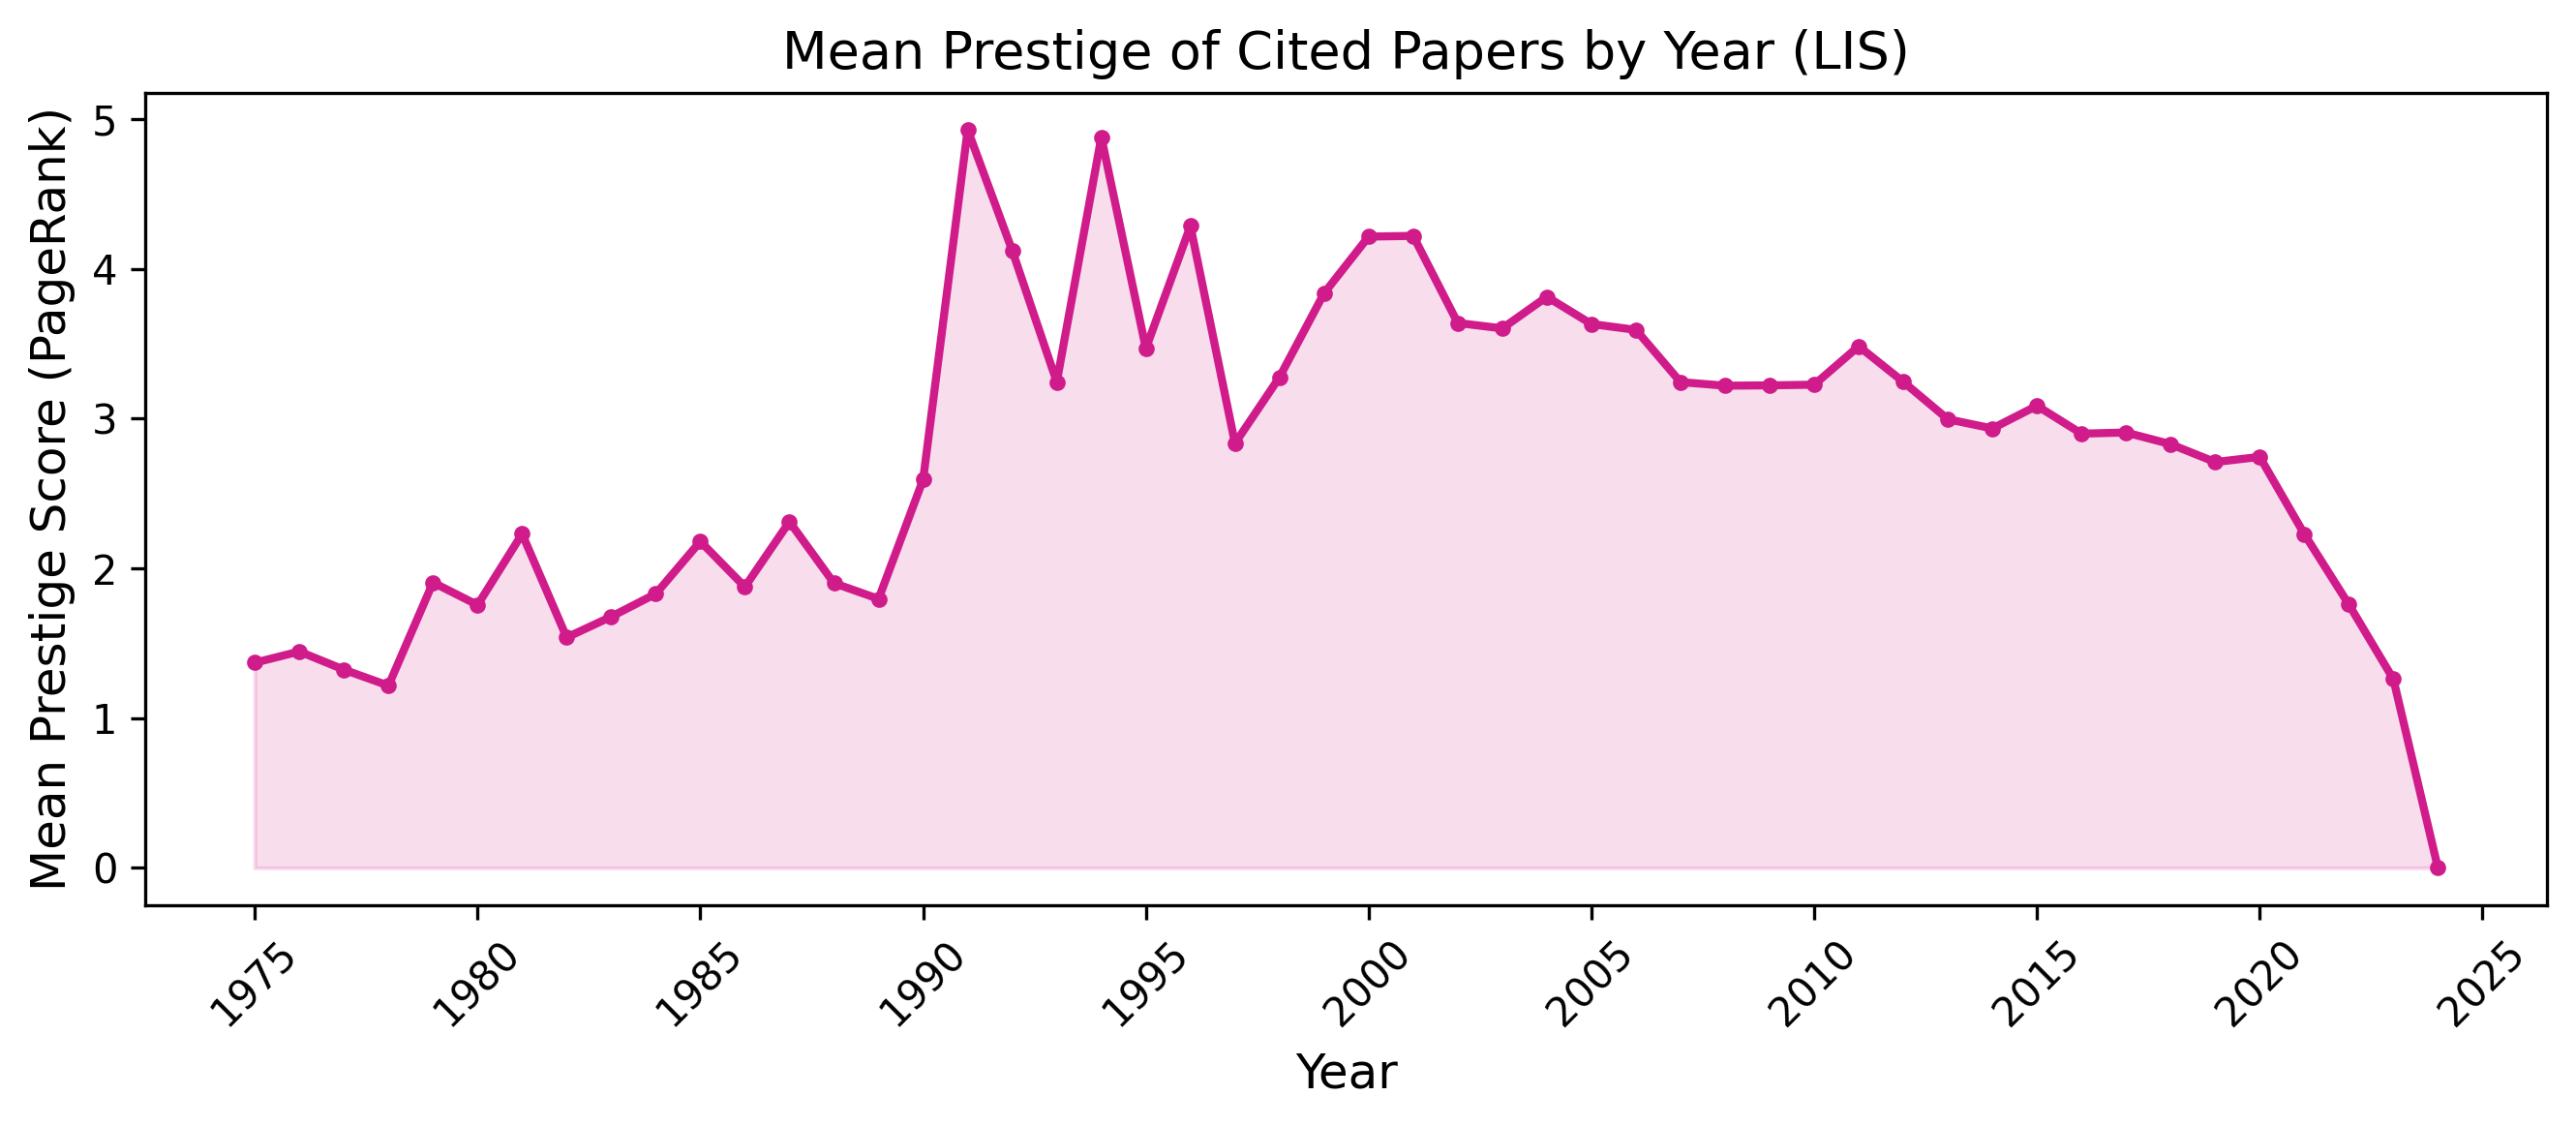
\includegraphics[width=0.75\textwidth]{../figures/dimensions/fig2_mean_citations_per_year.png}
\caption{Mean citations per year for LIS publications in the Dimensions dataset.}
\label{fig:dim_cites}
\end{figure}

Figure~\ref{fig:dim_cites} shows the mean citation count per publication year. Papers published in the 1990s and early 2000s have accumulated the highest mean citation counts, reflecting the combined effect of their age (more time to accumulate citations) and their foundational role in establishing the modern LIS research agenda. The decline in mean citations for more recent papers is expected, as these papers have had less time to accumulate citations.

\begin{figure}[h!]
\centering
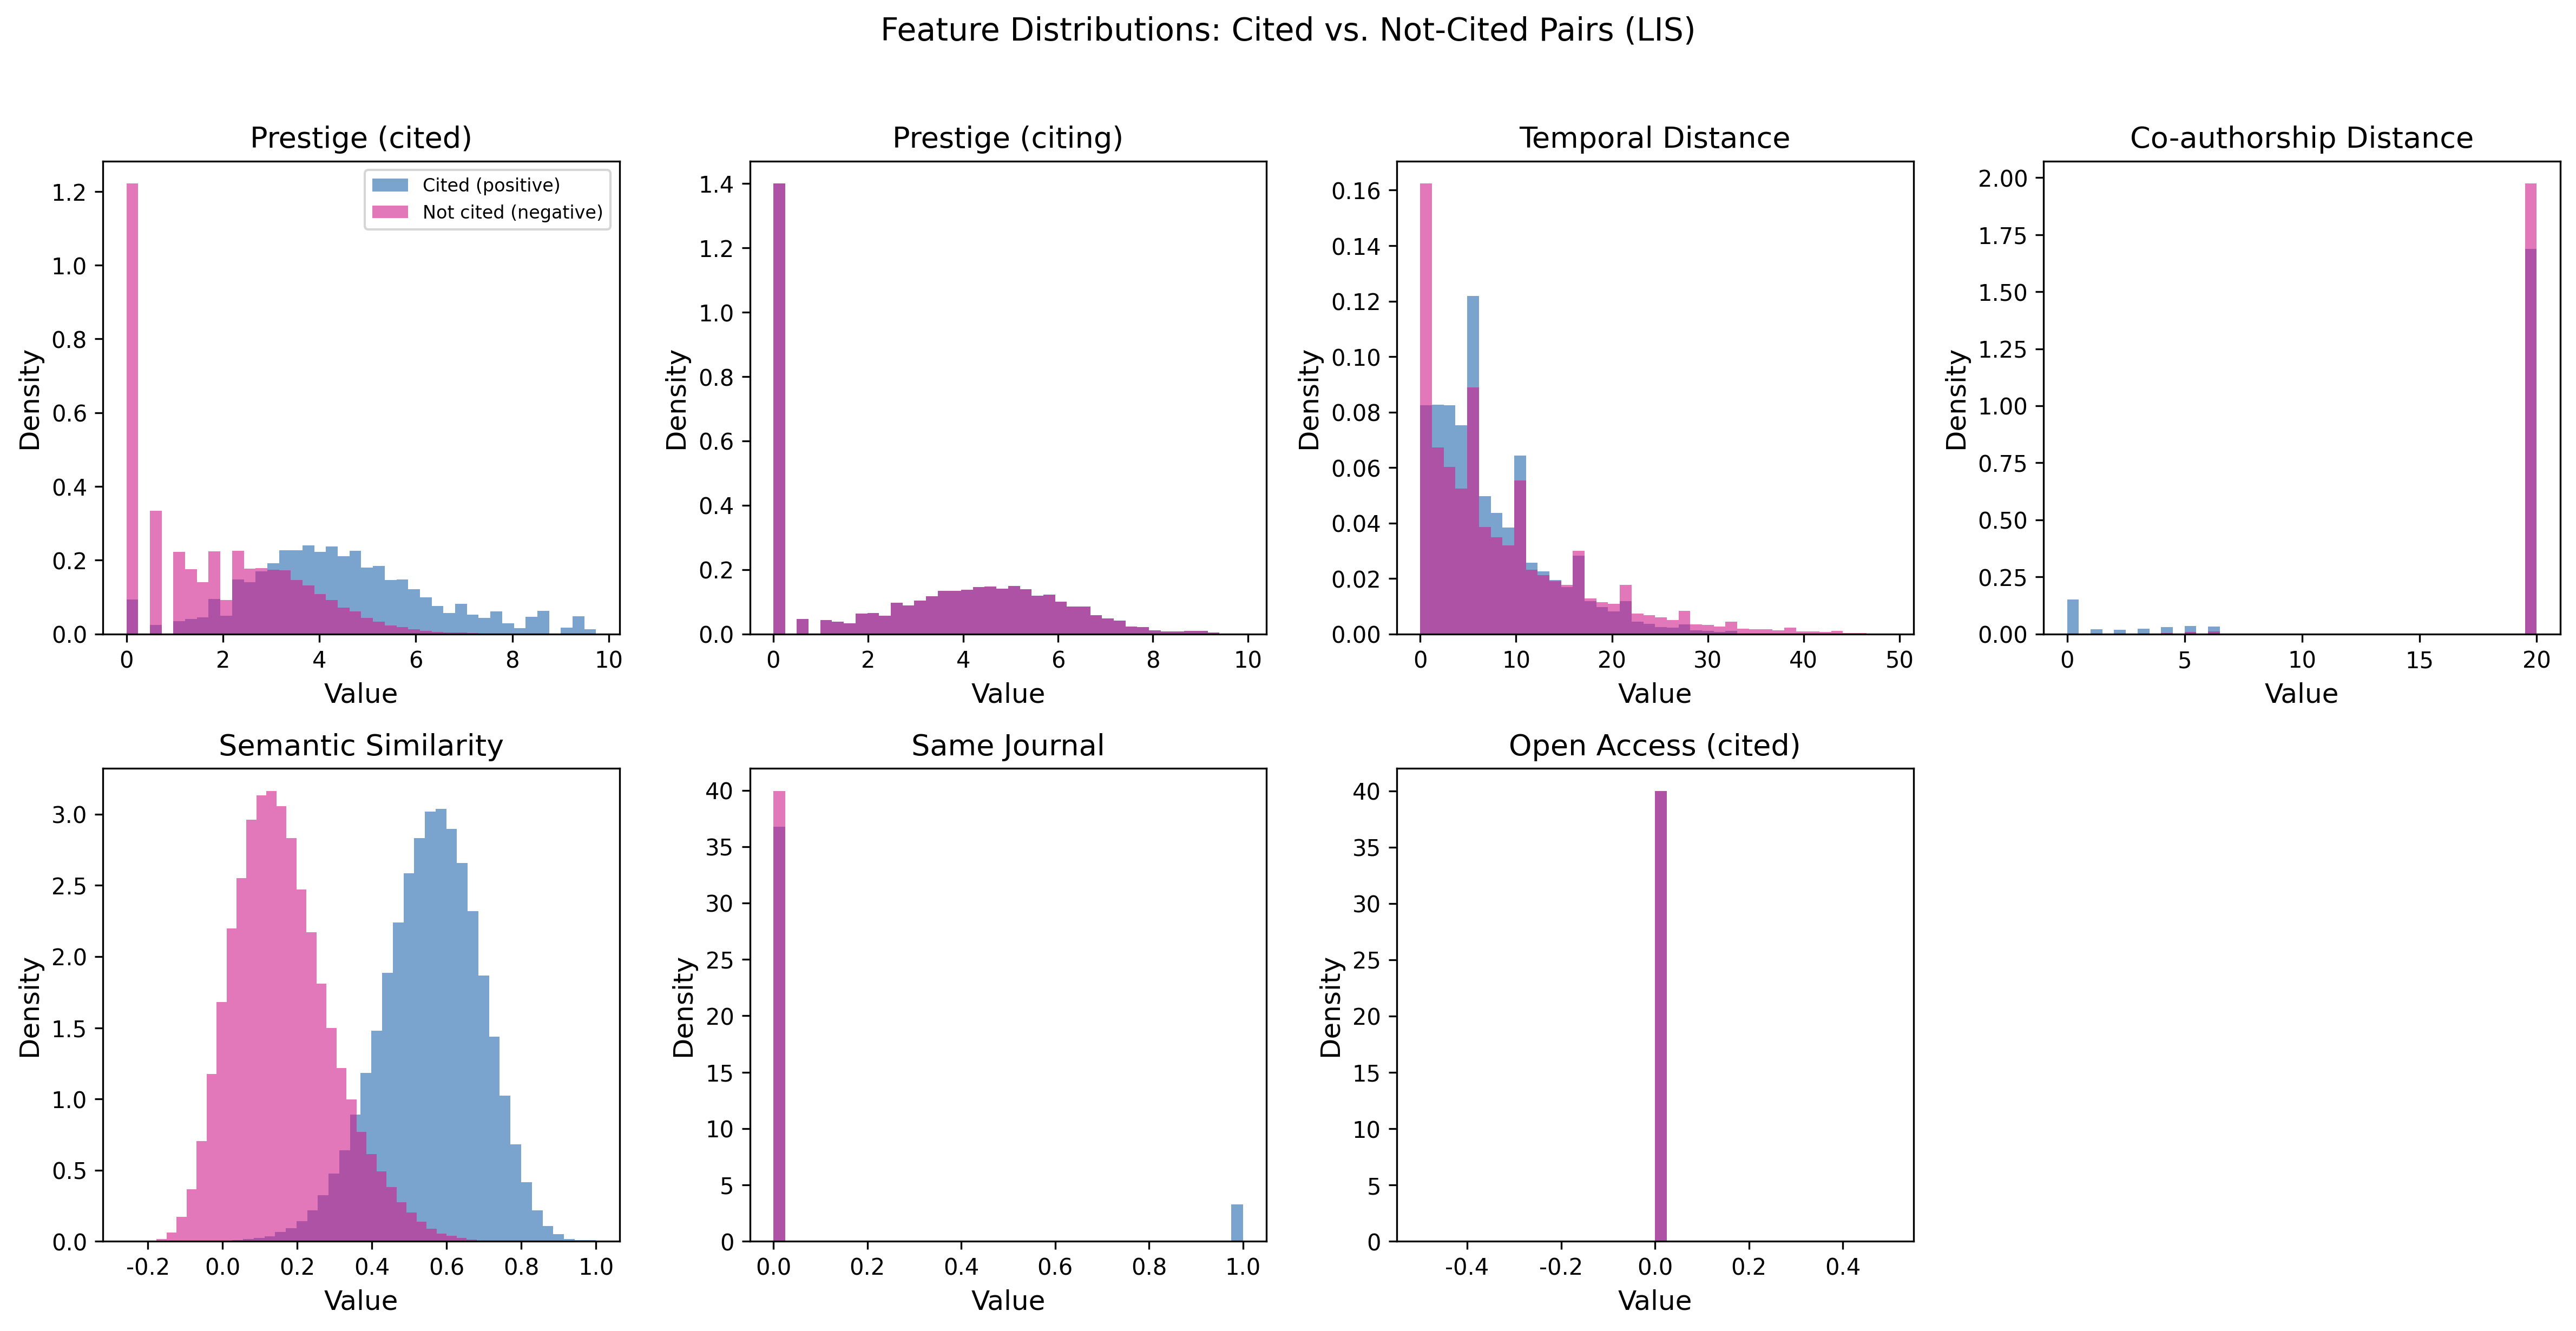
\includegraphics[width=0.75\textwidth]{../figures/dimensions/fig3_feature_distributions.png}
\caption{Distributions of key features for cited (positive) and not-cited (negative) pairs in the Dimensions dataset.}
\label{fig:dim_features}
\end{figure}

Figure~\ref{fig:dim_features} illustrates the distributions of key features for positive (cited) and negative (not-cited) pairs. The separation between the two distributions is most pronounced for semantic similarity and prestige of the cited paper, confirming that these features carry strong discriminative signal. The co-authorship distance distribution shows that cited pairs tend to have shorter social distances, though the overlap between distributions is substantial, reflecting the fact that many citations cross social boundaries.

\subsection{Model Performance}

We evaluated the six machine learning models on the 500,000 citation pairs from the Dimensions dataset. The results, summarized in Table~\ref{tab:dim_results}, demonstrate exceptionally high predictive accuracy across all models, with non-linear models showing a distinct advantage.

\begin{table}[h!]
\centering
\caption{Model Performance on Dimensions Dataset (5-Fold Stratified CV, Mean $\pm$ Std)}
\label{tab:dim_results}
\resizebox{\textwidth}{!}{
\begin{tabular}{lcccccc}
\toprule
\textbf{Model} & \textbf{ROC-AUC} & \textbf{F1} & \textbf{Accuracy} & \textbf{Precision} & \textbf{Recall} & \textbf{MCC} \\
\midrule
Logistic Regression & $0.9897 \pm 0.0002$ & $0.9522 \pm 0.0004$ & $0.9521 \pm 0.0004$ & $0.9505 \pm 0.0004$ & $0.9539 \pm 0.0006$ & $0.9042 \pm 0.0008$ \\
Linear SVM & $0.9897 \pm 0.0002$ & $0.9522 \pm 0.0004$ & $0.9521 \pm 0.0004$ & $0.9505 \pm 0.0004$ & $0.9540 \pm 0.0005$ & $0.9043 \pm 0.0007$ \\
k-NN ($k=5$) & $0.9773 \pm 0.0005$ & $0.9485 \pm 0.0005$ & $0.9483 \pm 0.0005$ & $0.9459 \pm 0.0008$ & $0.9511 \pm 0.0007$ & $0.8967 \pm 0.0011$ \\
Random Forest & $0.9873 \pm 0.0003$ & $0.9503 \pm 0.0006$ & $0.9502 \pm 0.0006$ & $0.9473 \pm 0.0007$ & $0.9533 \pm 0.0010$ & $0.9003 \pm 0.0013$ \\
Gradient Boosting & $0.9904 \pm 0.0002$ & $0.9542 \pm 0.0006$ & $0.9540 \pm 0.0006$ & $0.9511 \pm 0.0006$ & $0.9573 \pm 0.0008$ & $0.9081 \pm 0.0012$ \\
MLP Neural Network & $\mathbf{0.9906 \pm 0.0002}$ & $\mathbf{0.9540 \pm 0.0006}$ & $\mathbf{0.9539 \pm 0.0005}$ & $\mathbf{0.9518 \pm 0.0022}$ & $\mathbf{0.9562 \pm 0.0032}$ & $\mathbf{0.9078 \pm 0.0010}$ \\
\bottomrule
\end{tabular}}
\end{table}

The MLP Neural Network achieved the highest ROC-AUC (0.9906), closely followed by Gradient Boosting (0.9904). The performance gap between the best model and the linear baseline (Logistic Regression, AUC 0.9897) is modest but consistent, suggesting that the feature space is largely linearly separable, with non-linear models capturing additional variance at the margins. Even the weakest model (k-NN, AUC 0.9773) achieves performance that would be considered exceptional in most classification tasks, underscoring the high predictability of citation dynamics in this corpus.

The near-identical performance of Logistic Regression and Linear SVM (both AUC 0.9897) is noteworthy. These two models optimize different objective functions (log-likelihood vs. hinge loss) but arrive at essentially the same decision boundary, suggesting that the linear component of the feature-label relationship is highly robust and not sensitive to the specific loss function used.

\begin{figure}[h!]
\centering
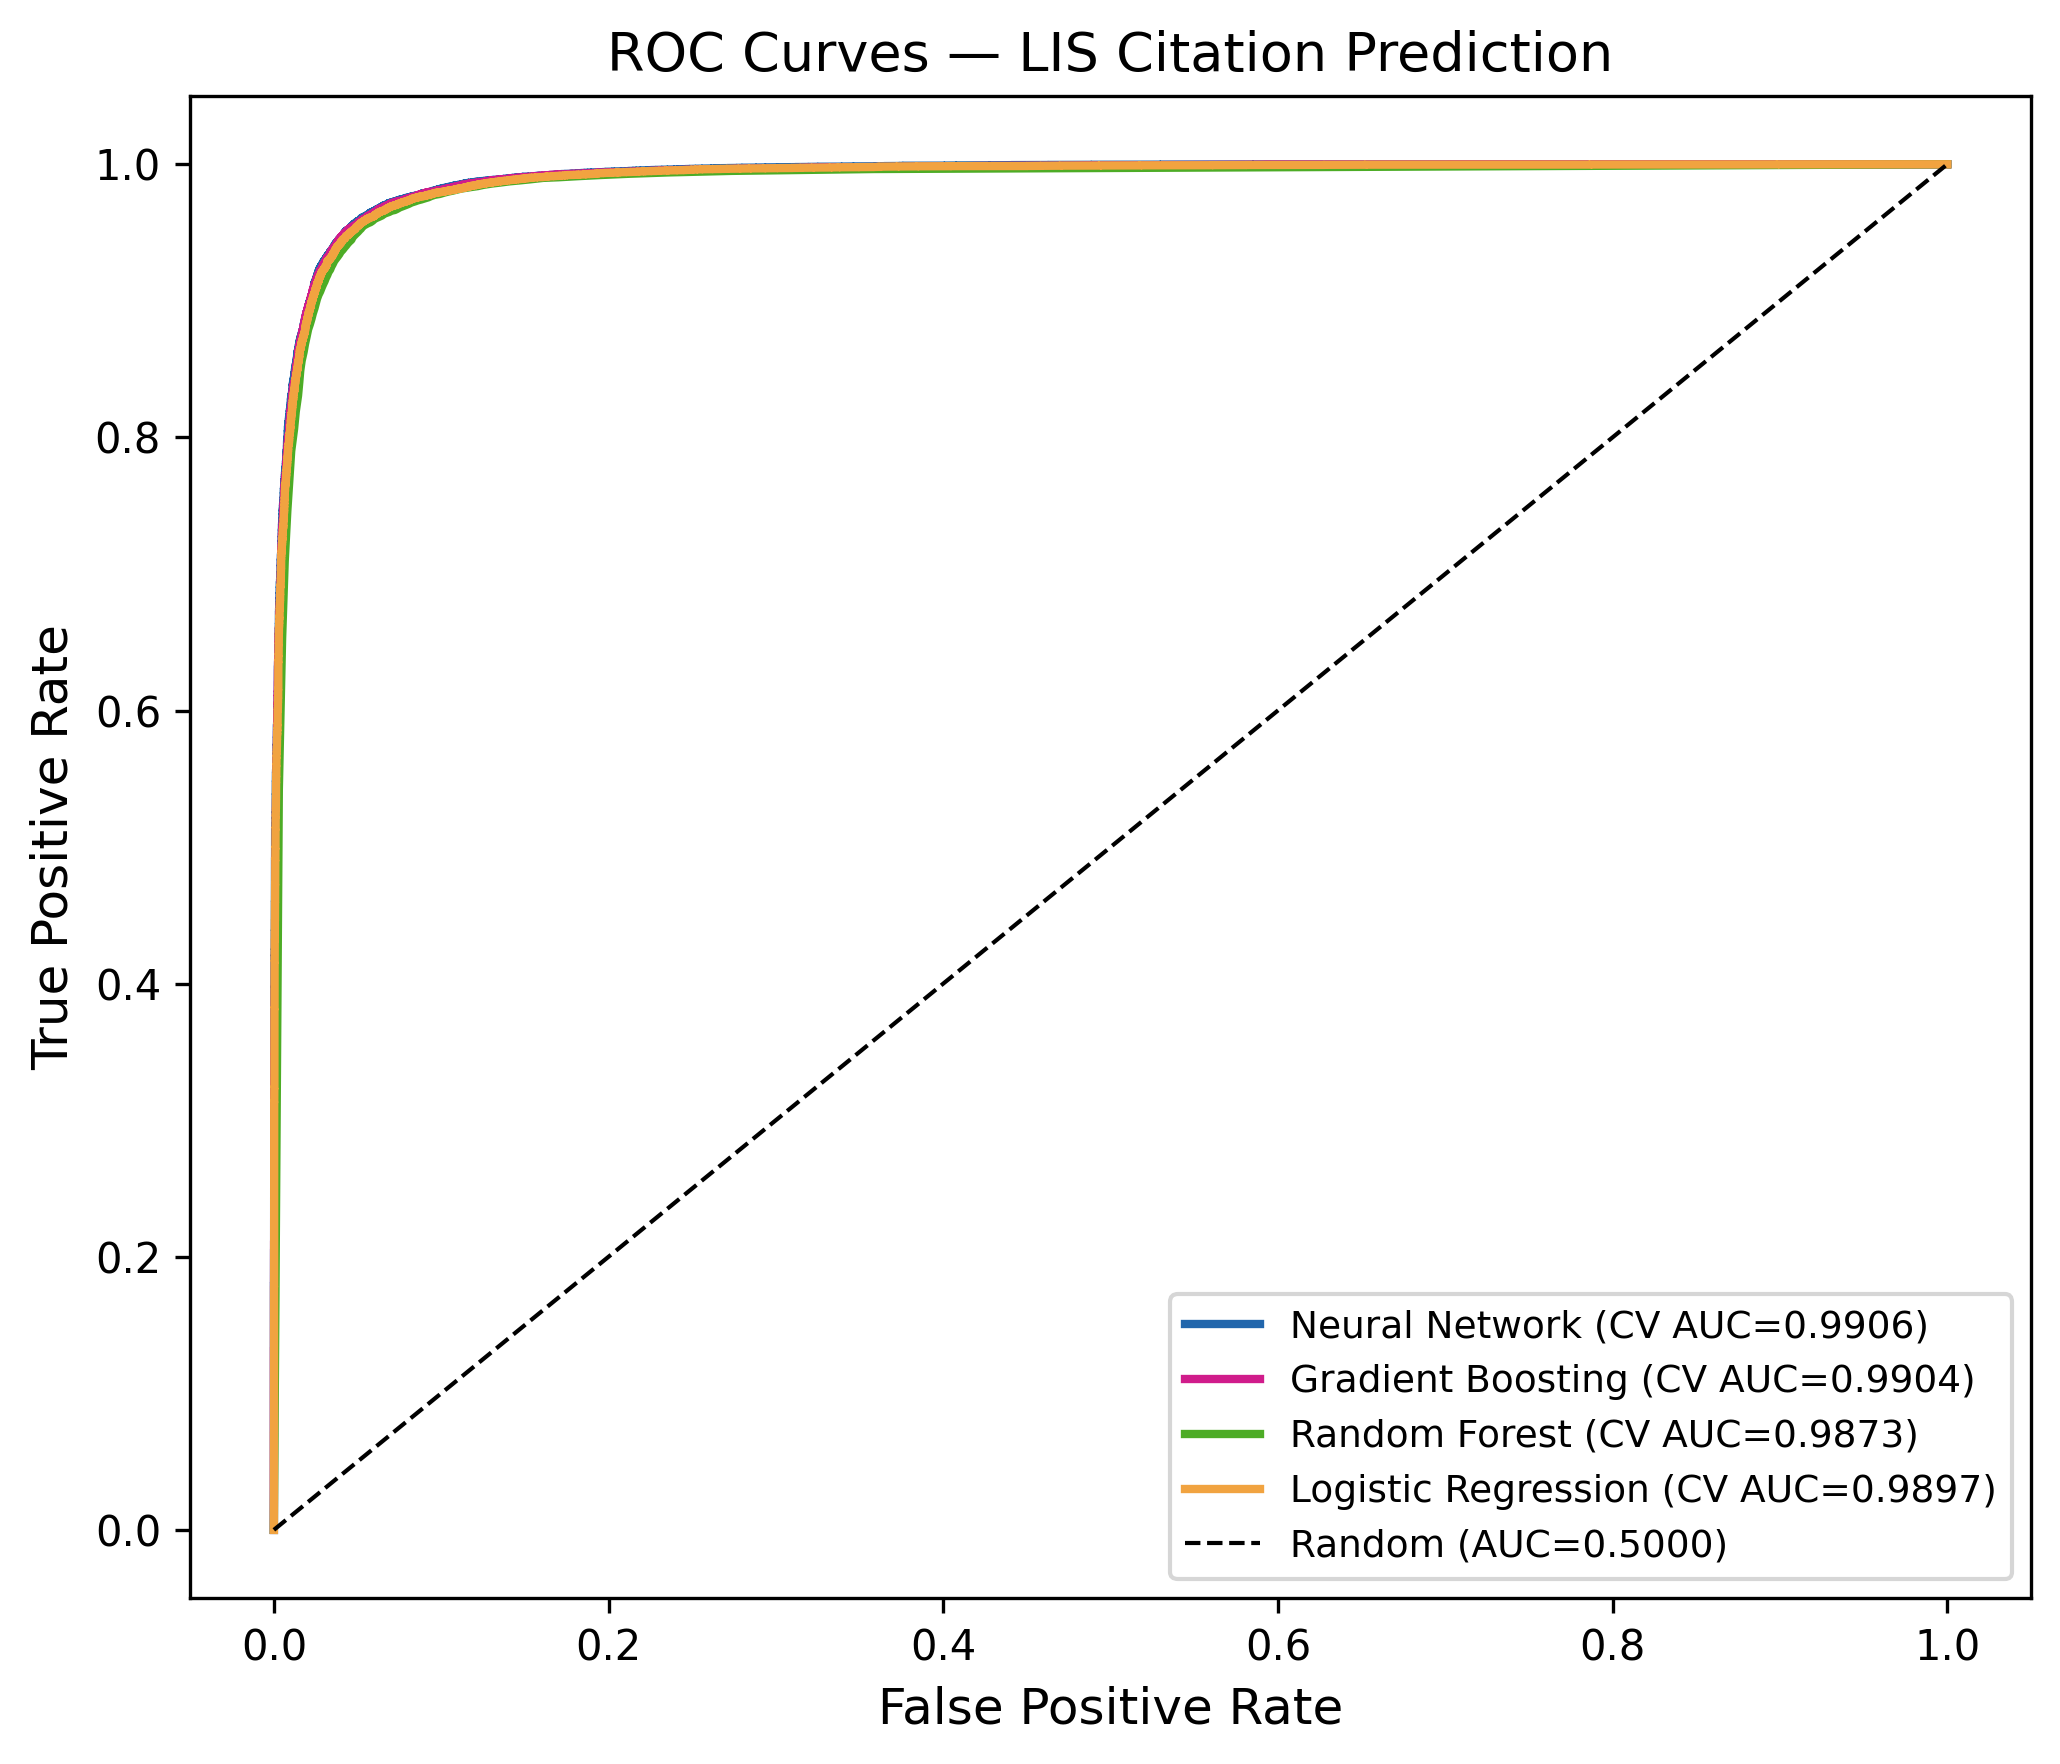
\includegraphics[width=0.75\textwidth]{../figures/dimensions/fig5_roc_curves.png}
\caption{ROC curves for all models evaluated on the Dimensions dataset.}
\label{fig:dim_roc}
\end{figure}

Figure~\ref{fig:dim_roc} shows the ROC curves for all six models. The curves are tightly clustered near the top-left corner of the ROC space, reflecting the high overall performance. The separation between models is most visible at low false positive rates, where the ensemble methods and neural network maintain higher true positive rates than the linear models.

\begin{figure}[h!]
\centering
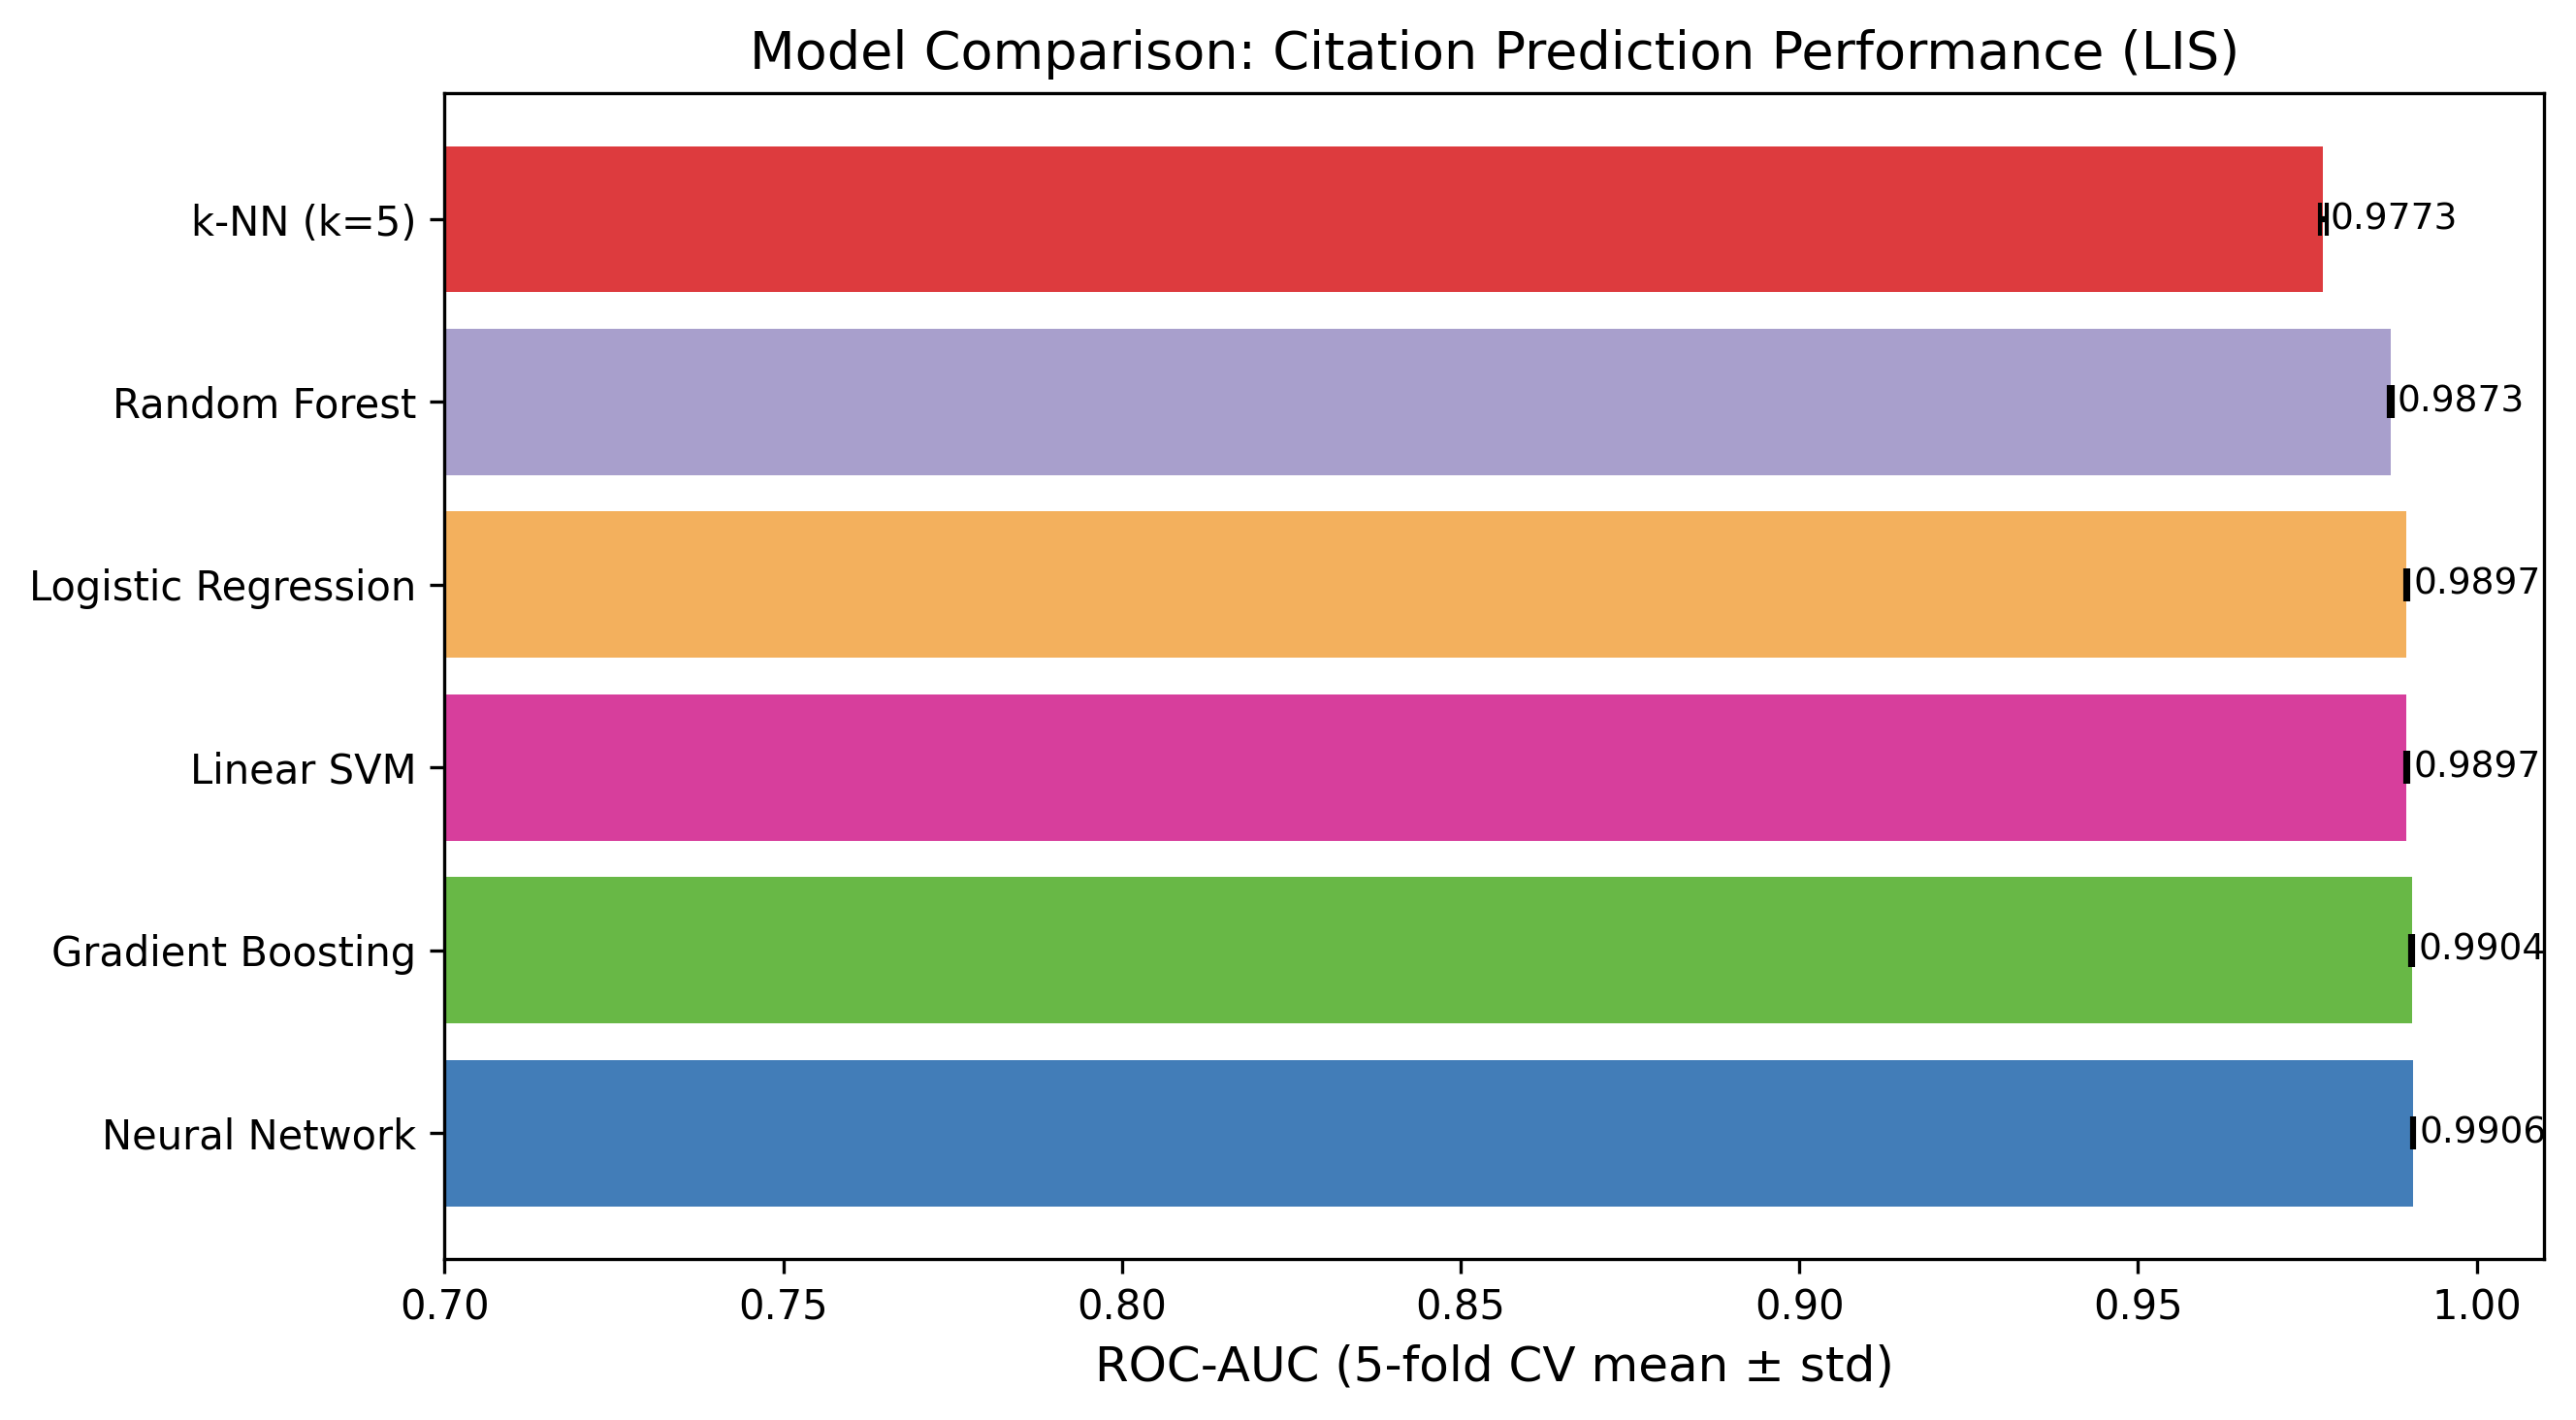
\includegraphics[width=0.75\textwidth]{../figures/dimensions/fig4_model_comparison.png}
\caption{Model comparison across all six performance metrics on the Dimensions dataset.}
\label{fig:dim_compare}
\end{figure}

\subsection{Feature Importance and Explainability}

\subsubsection{SHAP Analysis}

To understand the drivers of citation within the Dimensions dataset, we analyzed SHAP values \citep{lundberg2017unified} for the best-performing model. The SHAP analysis revealed that \textbf{Semantic Similarity} is the most dominant predictor (mean absolute SHAP value $\approx 0.305$), followed by the \textbf{Prestige of the Cited Paper} ($\approx 0.137$). Co-authorship distance ($\approx 0.022$) and temporal distance ($\approx 0.017$) played secondary roles. The prestige of the citing paper ($\approx 0.013$) and same-journal indicator ($\approx 0.014$) contributed modestly.

\begin{figure}[h!]
\centering
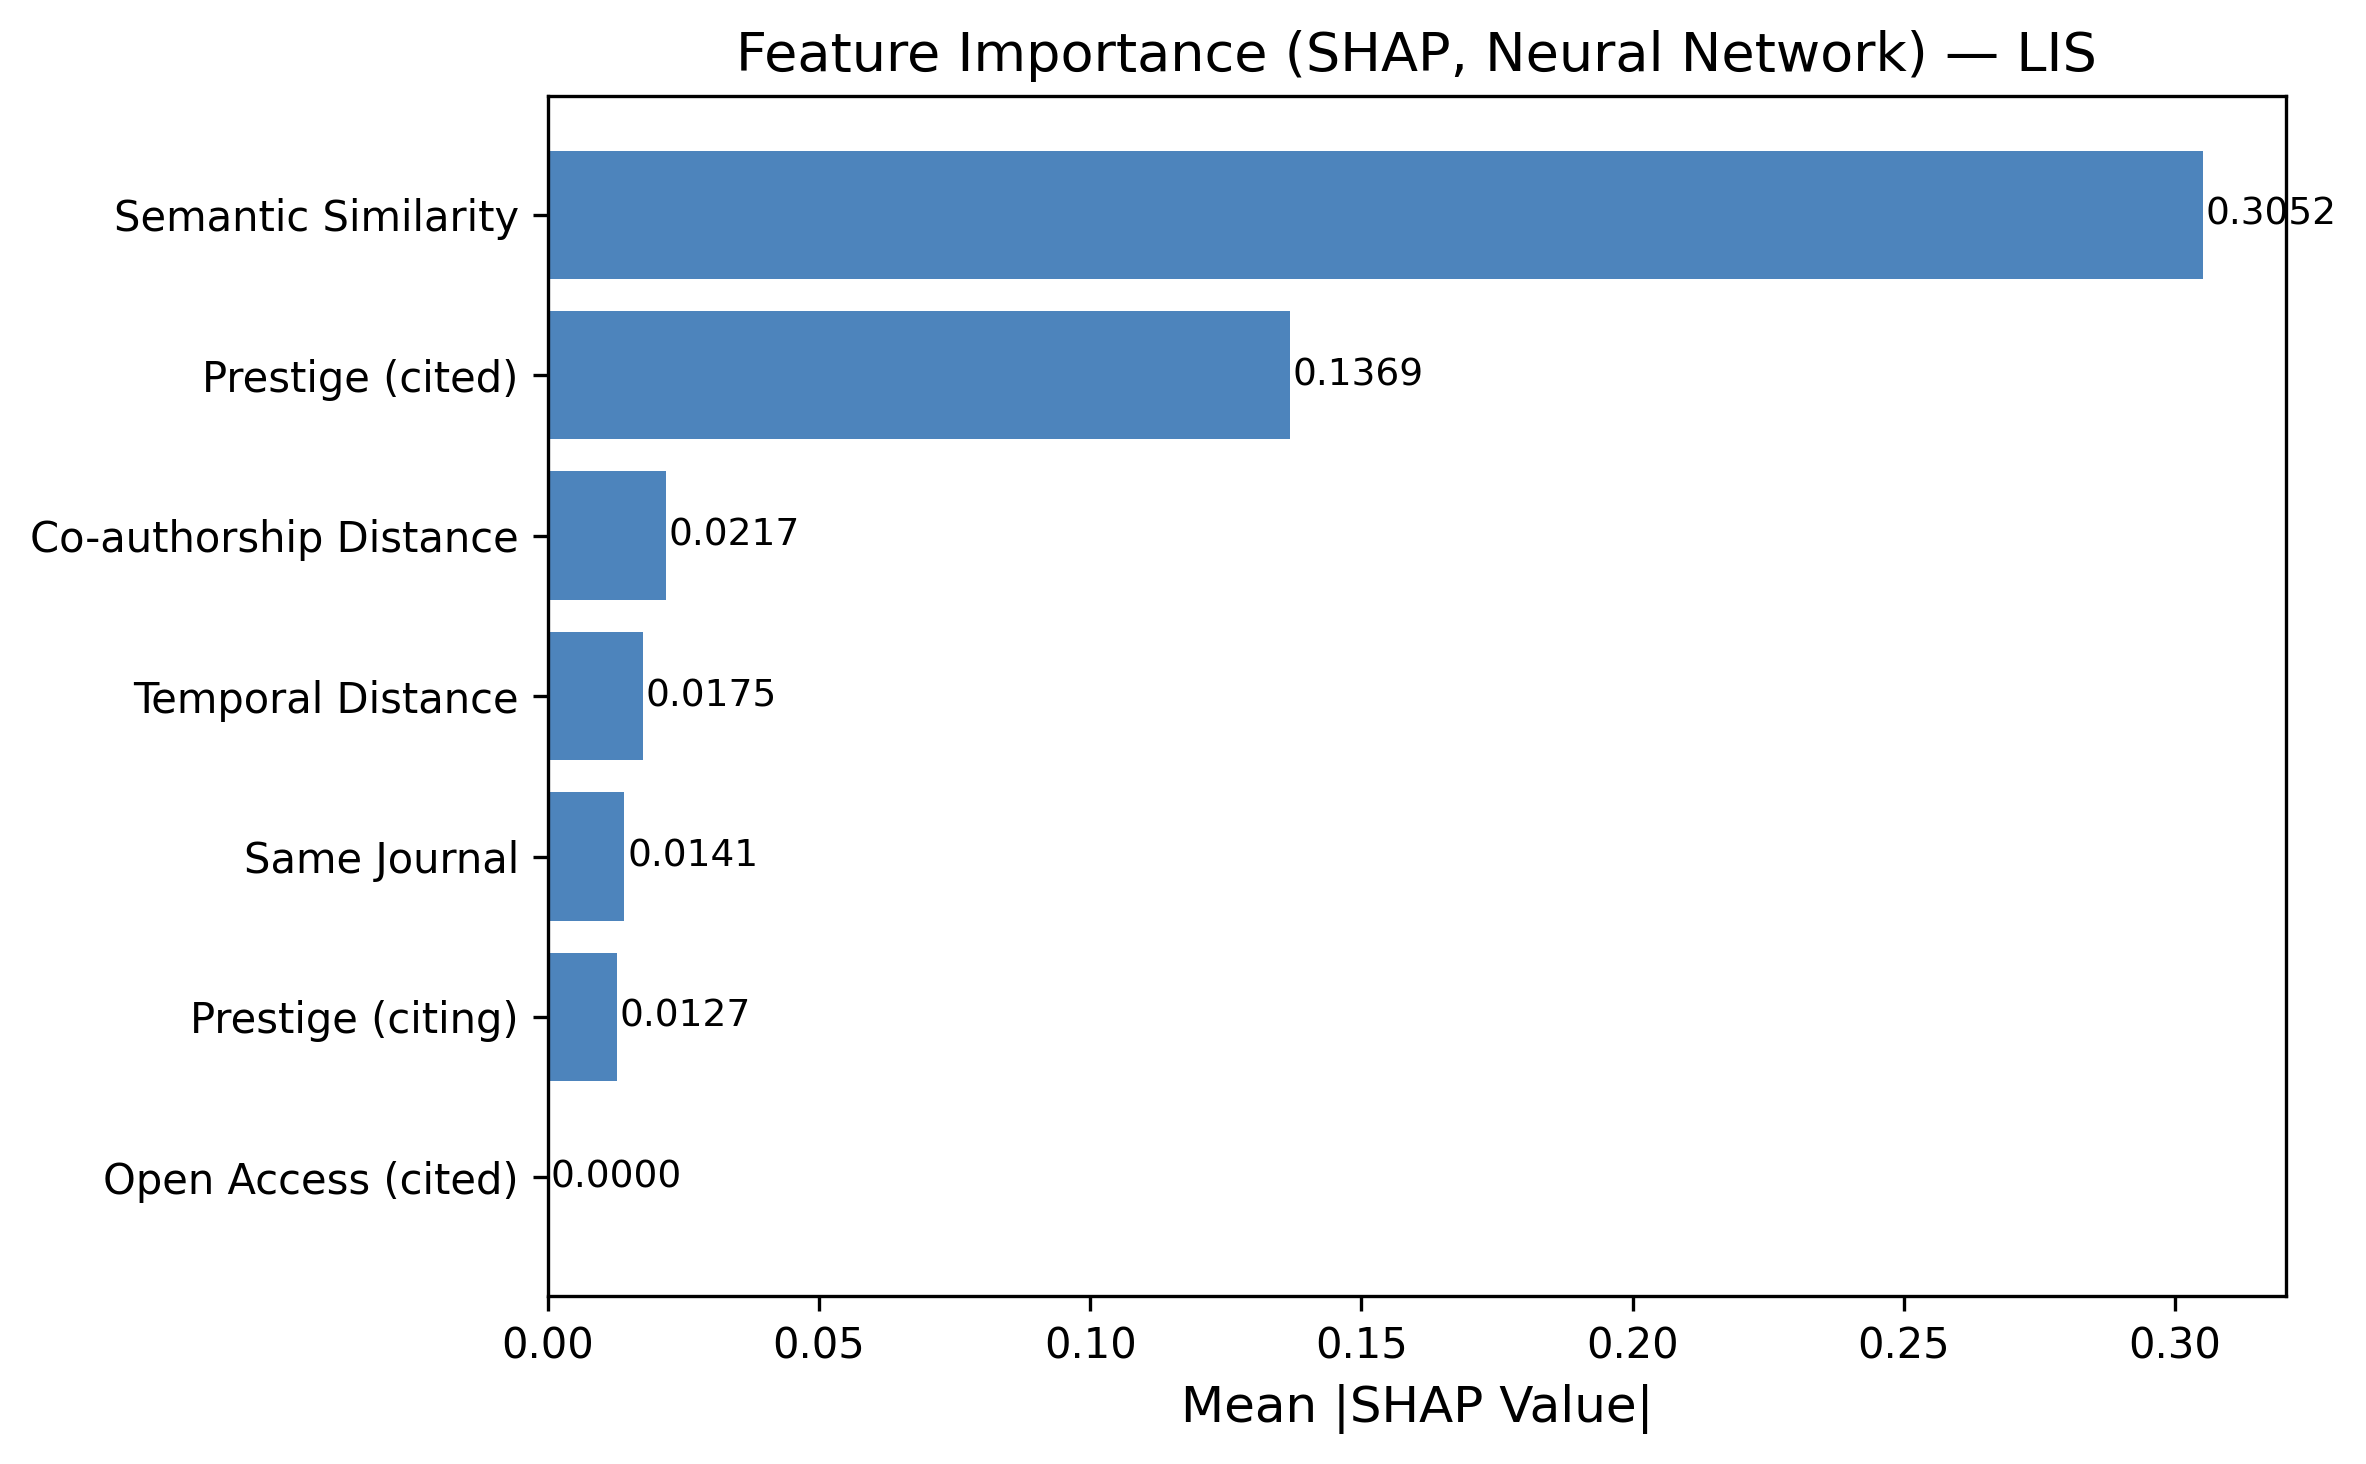
\includegraphics[width=0.75\textwidth]{../figures/dimensions/fig6_shap_importance.png}
\caption{Mean absolute SHAP values for the best model on the Dimensions dataset.}
\label{fig:dim_shap}
\end{figure}

This finding suggests that while the Matthew effect (prestige) is present and significant, the actual content relevance (semantics) is the primary driver of citations in this corpus. Papers are cited primarily because they are topically relevant to the citing paper, not merely because they are famous. This result aligns with the ``Citation proximus'' findings of Kozlowski et al. \citep{kozlowski2025citation}, who found that semantic proximity rivals prestige in predicting citations.

The relatively modest contribution of co-authorship distance (SHAP $\approx 0.022$) is surprising given the strong theoretical and empirical evidence for social proximity effects in citation behavior. One possible explanation is that in LIS, a relatively small and interconnected field, the co-authorship network is dense enough that most pairs of authors are within a few steps of each other, reducing the discriminative power of this feature. Another possibility is that the social proximity effect is largely mediated by semantic similarity: researchers who collaborate tend to work on similar topics, and it is the topical similarity rather than the social connection per se that drives citation.

\subsubsection{Ablation Study}

To rigorously quantify the contribution of different feature classes, we conducted an ablation study using the Random Forest model. Table~\ref{tab:dim_ablation} reports the ROC-AUC for models trained on various feature subsets.

\begin{table}[h!]
\centering
\caption{Feature Ablation Study (Dimensions Dataset, Random Forest)}
\label{tab:dim_ablation}
\begin{tabular}{lcc}
\toprule
\textbf{Feature Subset} & \textbf{ROC-AUC} & \textbf{Drop from All Features} \\
\midrule
All features & 0.9868 & -- \\
No semantic similarity & 0.8709 & $-0.1159$ \\
No co-authorship distance & 0.9859 & $-0.0009$ \\
No prestige & 0.9618 & $-0.0250$ \\
Semantic similarity only & 0.9513 & $-0.0355$ \\
Network features only & 0.8512 & $-0.1356$ \\
Temporal + semantic & 0.9576 & $-0.0292$ \\
\bottomrule
\end{tabular}
\end{table}

The ablation results confirm and amplify the SHAP findings. Removing semantic similarity causes the most severe performance drop (AUC falls from 0.9868 to 0.8709, a drop of 0.1159). Removing prestige features causes a more modest but still substantial drop (0.0250). Removing co-authorship distance has a negligible effect (0.0009), suggesting that the social proximity signal is largely subsumed by the semantic and prestige features in this dataset.

Notably, a model trained on semantic similarity alone achieves an AUC of 0.9513, substantially outperforming a model trained on all network features combined (AUC 0.8512). This finding has important implications for the design of citation prediction systems: high-quality semantic embeddings may be sufficient to achieve near-optimal performance, reducing the need for expensive network construction.

The combination of semantic similarity and temporal distance (AUC 0.9576) achieves performance close to the full model (0.9868), suggesting that these two features capture the majority of the predictive signal. The additional features (prestige, co-authorship distance) provide incremental improvements that, while statistically significant, are modest in absolute terms.

%% ============================================================
\section{Results: OpenAlex Analysis}
\label{sec:oa}
%% ============================================================

\subsection{Corpus Overview}

The OpenAlex dataset covers a longer time span (1975--2024) and provides a complementary perspective on LIS citation dynamics. Figure~\ref{fig:oa_pubs} shows the temporal distribution of publications, exhibiting exponential growth from the late 1990s onward, reflecting both the expansion of LIS research and the increasing coverage of OpenAlex over time.

\begin{figure}[h!]
\centering
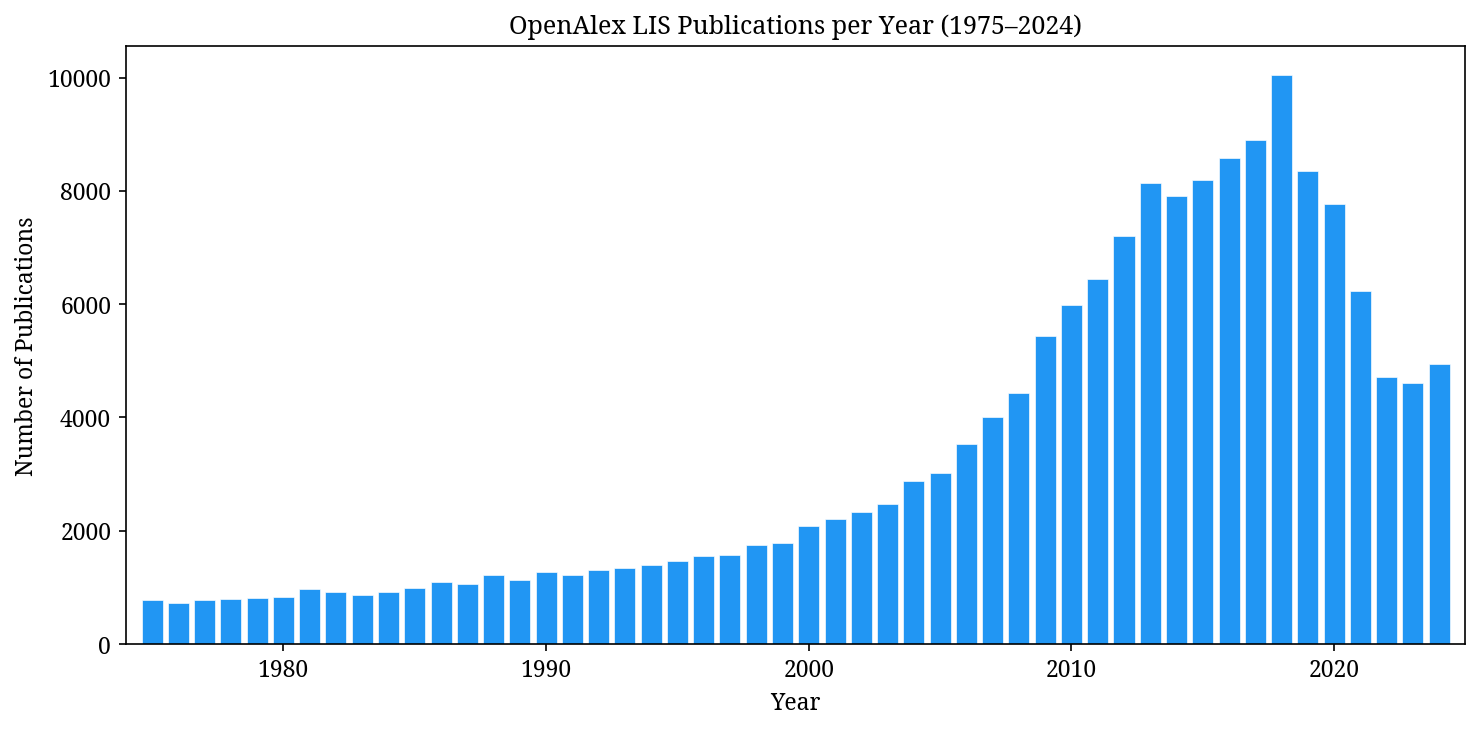
\includegraphics[width=0.75\textwidth]{../figures/oa/oa_fig1_publications_per_year.png}
\caption{Number of LIS publications per year in the OpenAlex dataset (1975--2024).}
\label{fig:oa_pubs}
\end{figure}

\begin{figure}[h!]
\centering
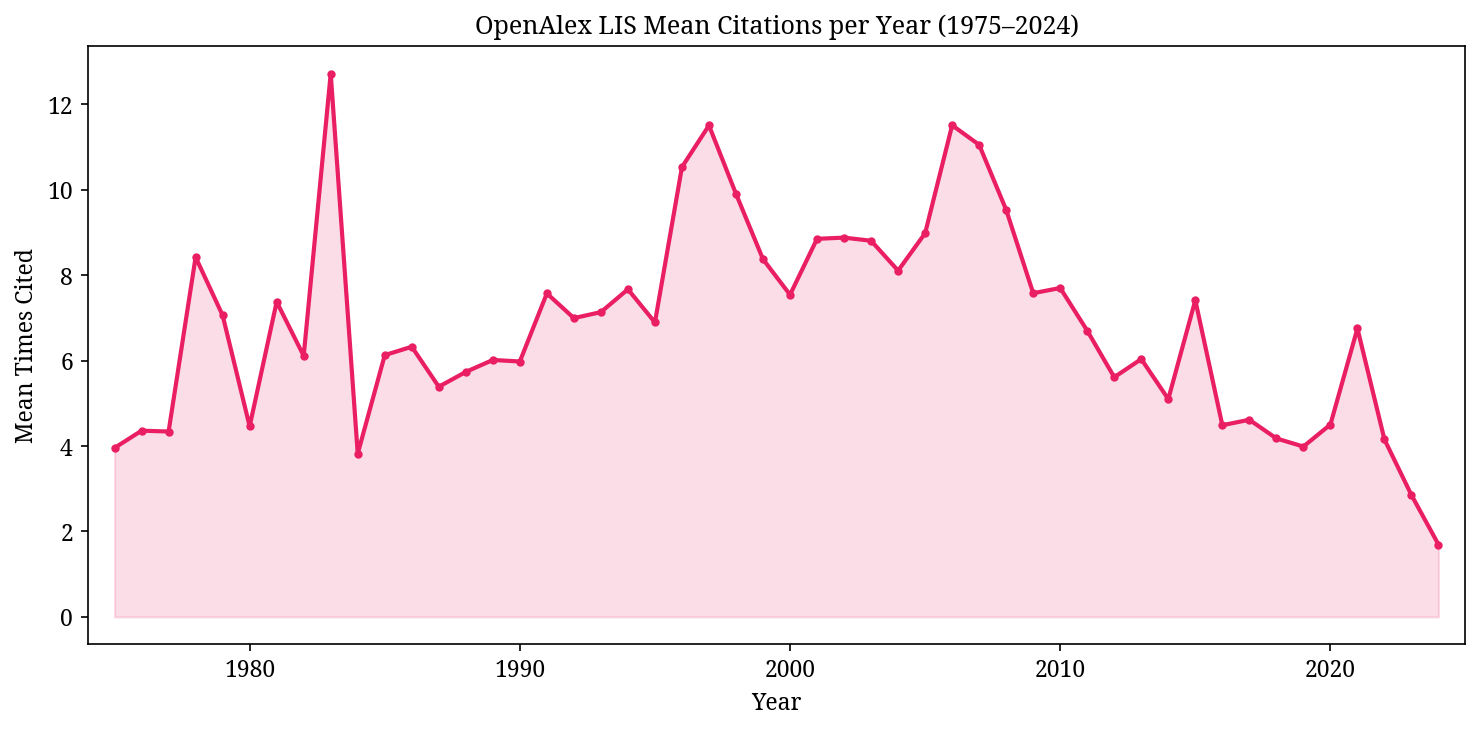
\includegraphics[width=0.75\textwidth]{../figures/oa/oa_fig2_mean_citations_per_year.png}
\caption{Mean citations per year for LIS publications in the OpenAlex dataset.}
\label{fig:oa_cites}
\end{figure}

Figure~\ref{fig:oa_cites} shows the mean citation count per publication year in the OpenAlex dataset. The pattern is broadly similar to Dimensions, with older papers having accumulated more citations on average. However, the OpenAlex dataset shows a more pronounced peak in the early 2000s, reflecting the rapid growth of the digital library and information retrieval literature during this period.

\begin{figure}[h!]
\centering
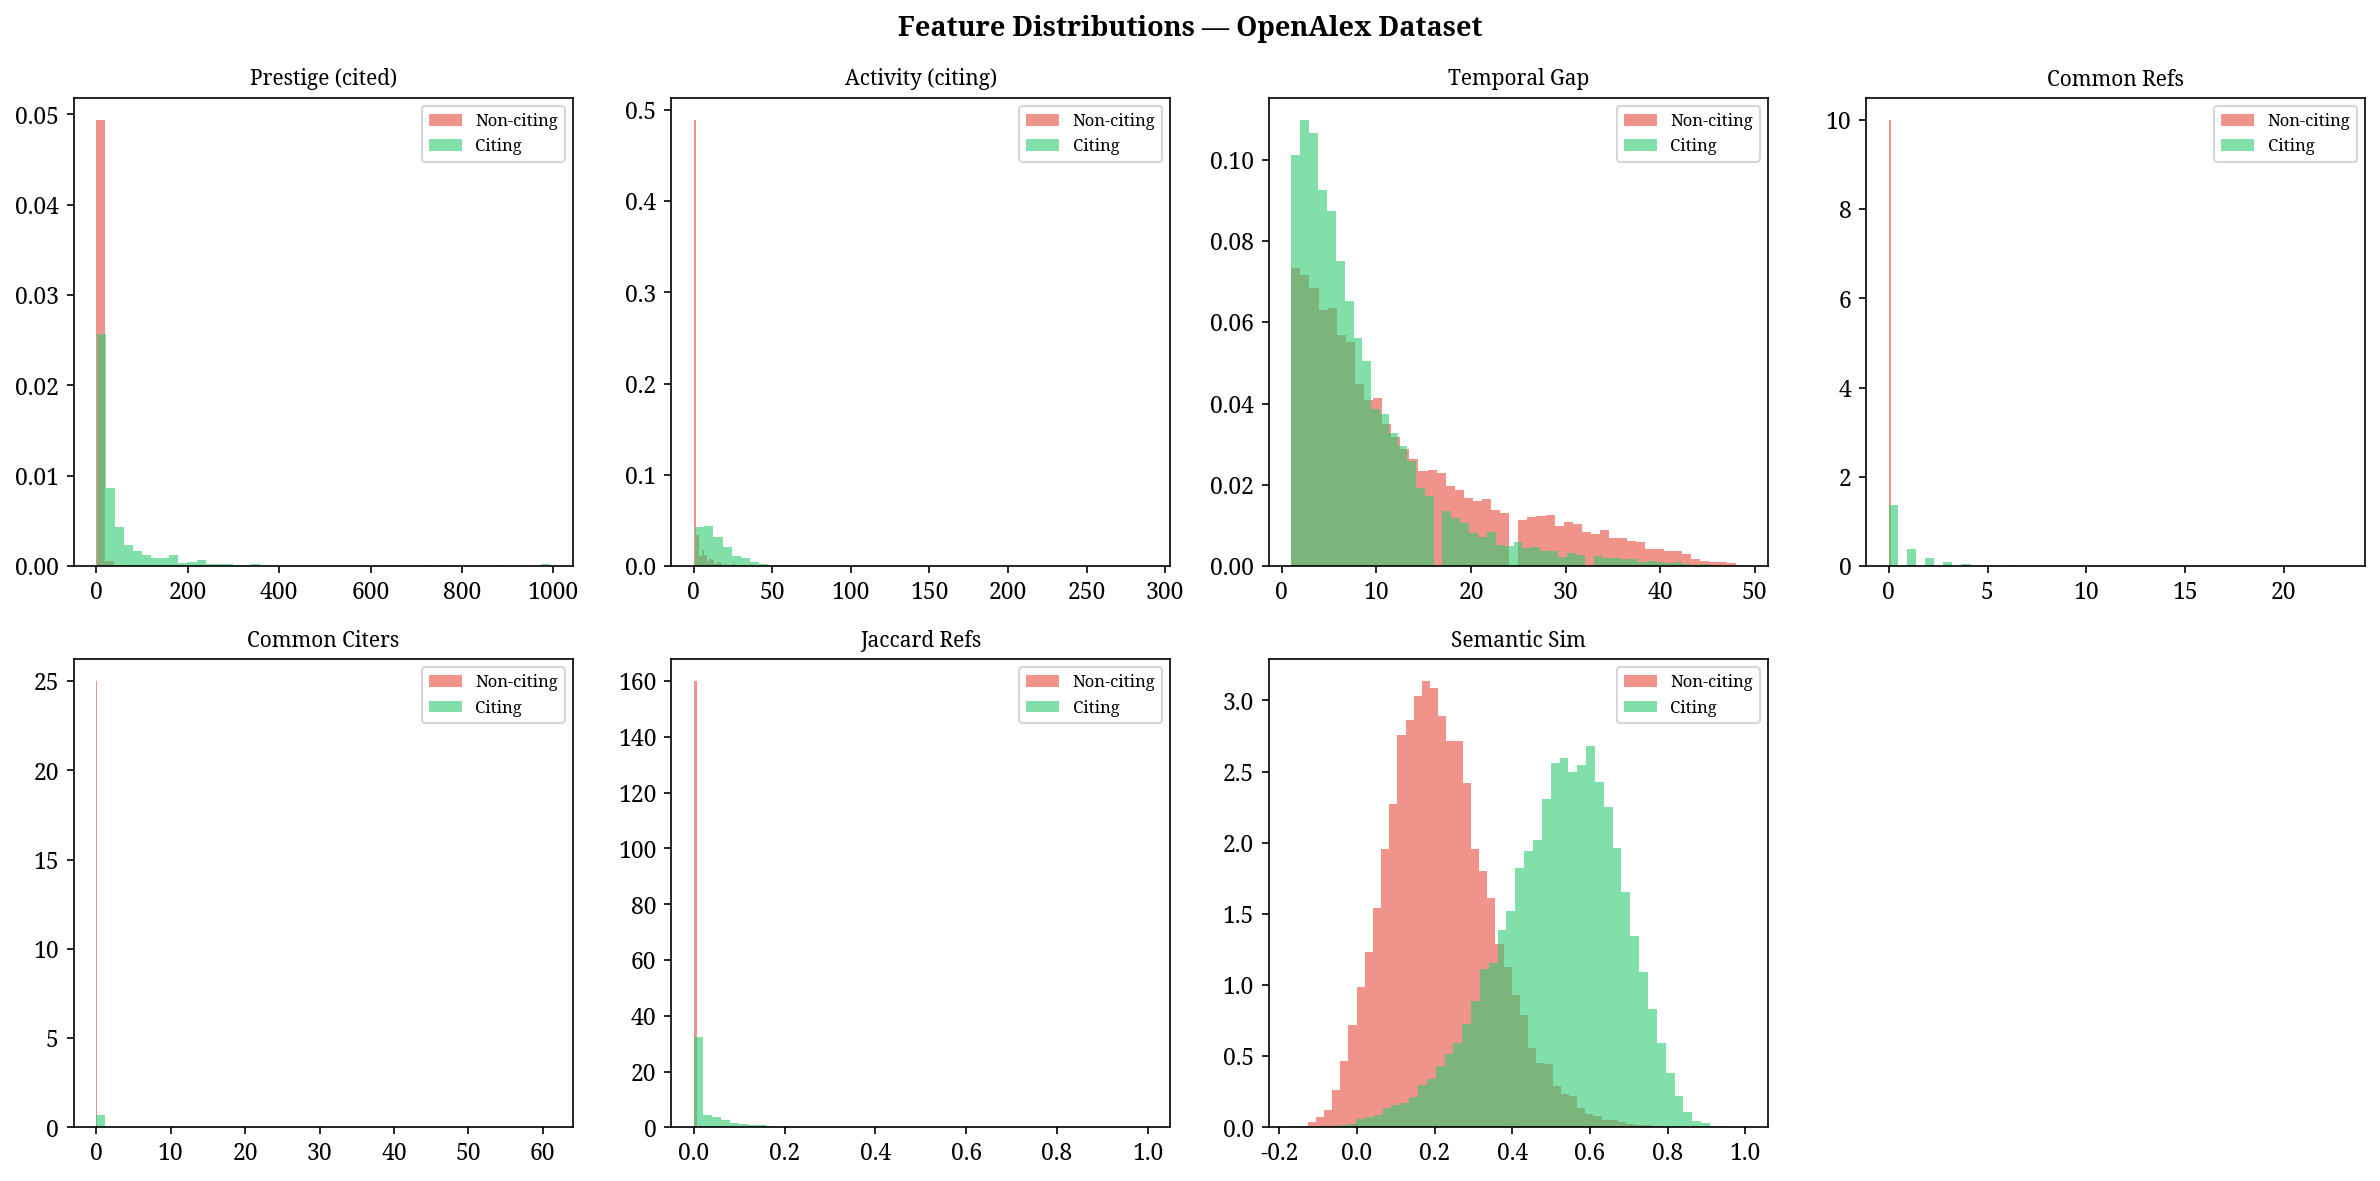
\includegraphics[width=0.75\textwidth]{../figures/oa/oa_fig3_feature_distributions.png}
\caption{Distributions of key features for cited (positive) and not-cited (negative) pairs in the OpenAlex dataset.}
\label{fig:oa_features}
\end{figure}

Figure~\ref{fig:oa_features} shows the feature distributions for the OpenAlex dataset. As with Dimensions, the separation between positive and negative pairs is most pronounced for semantic similarity and prestige. The reference overlap features (common references, Jaccard similarity) also show clear separation, reflecting the tendency for papers that share a common intellectual heritage to cite each other.

\begin{figure}[h!]
\centering
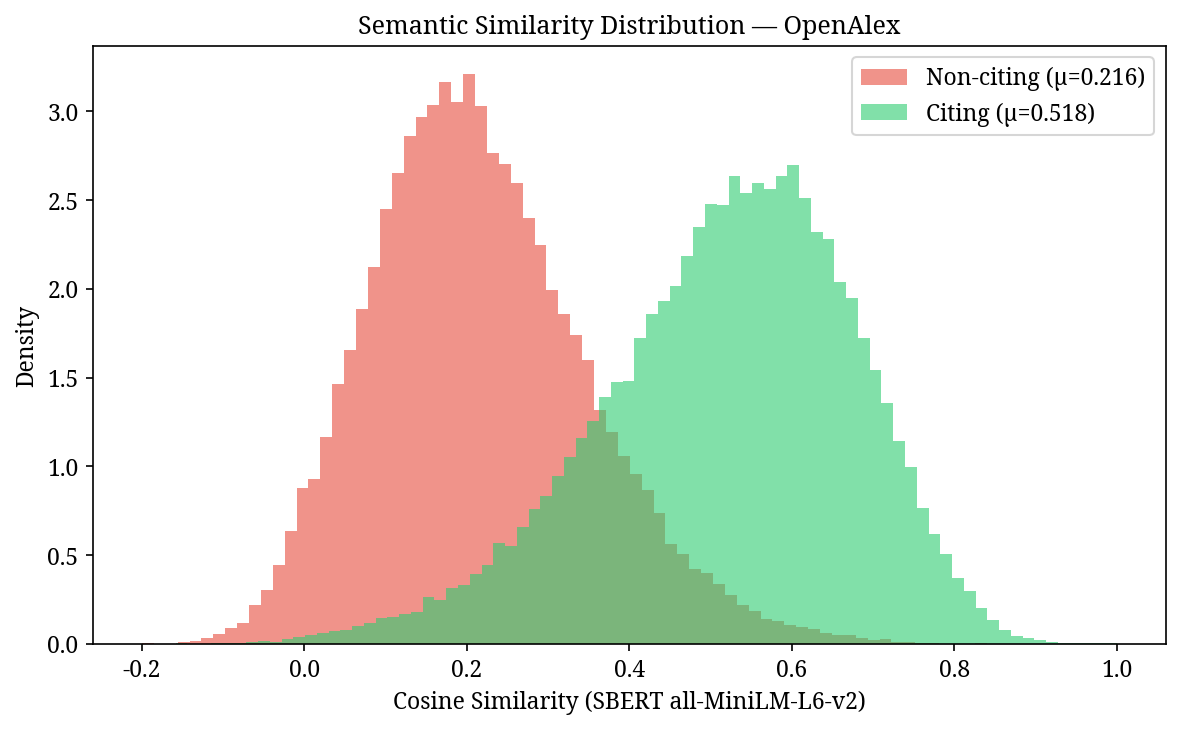
\includegraphics[width=0.75\textwidth]{../figures/oa/oa_fig8_semantic_sim.png}
\caption{Semantic similarity distributions for cited and not-cited pairs in the OpenAlex dataset. Mean similarity: positive pairs = 0.5183, negative pairs = 0.2161.}
\label{fig:oa_sem}
\end{figure}

Figure~\ref{fig:oa_sem} shows the semantic similarity distributions in detail. The mean semantic similarity for positive pairs (0.5183) is substantially higher than for negative pairs (0.2161), confirming the strong discriminative power of this feature. The distributions overlap substantially, however, indicating that many citations occur between papers with low semantic similarity (cross-disciplinary citations, methodological citations) and that many non-citations occur between papers with high semantic similarity (parallel but non-interacting research streams).

\subsection{Model Performance}

We evaluated four machine learning models on the 489,349 citation pairs from the OpenAlex dataset. Due to memory constraints associated with the scale of the dataset, k-NN and Neural Network models were excluded; the remaining four models were evaluated. The results are presented in Table~\ref{tab:oa_results}.

\begin{table}[h!]
\centering
\caption{Model Performance on OpenAlex Dataset (5-Fold Stratified CV, Mean $\pm$ Std)}
\label{tab:oa_results}
\resizebox{\textwidth}{!}{
\begin{tabular}{lcccccc}
\toprule
\textbf{Model} & \textbf{ROC-AUC} & \textbf{F1} & \textbf{Accuracy} & \textbf{Precision} & \textbf{Recall} & \textbf{MCC} \\
\midrule
Logistic Regression & $0.9872 \pm 0.0002$ & $0.9478 \pm 0.0004$ & $0.9495 \pm 0.0004$ & $0.9574 \pm 0.0013$ & $0.9385 \pm 0.0008$ & $0.8991 \pm 0.0008$ \\
Linear SVM & $0.9863 \pm 0.0003$ & $0.9451 \pm 0.0005$ & $0.9468 \pm 0.0005$ & $0.9549 \pm 0.0014$ & $0.9355 \pm 0.0011$ & $0.8937 \pm 0.0010$ \\
Random Forest & $0.9972 \pm 0.0001$ & $0.9793 \pm 0.0002$ & $0.9796 \pm 0.0002$ & $0.9729 \pm 0.0006$ & $0.9857 \pm 0.0005$ & $0.9592 \pm 0.0003$ \\
Gradient Boosting & $\mathbf{0.9979 \pm 0.0001}$ & $\mathbf{0.9810 \pm 0.0004}$ & $\mathbf{0.9813 \pm 0.0004}$ & $\mathbf{0.9752 \pm 0.0006}$ & $\mathbf{0.9868 \pm 0.0005}$ & $\mathbf{0.9626 \pm 0.0007}$ \\
\bottomrule
\end{tabular}}
\end{table}

The results on the OpenAlex dataset are striking in two respects. First, the overall performance is even higher than on Dimensions, with Gradient Boosting achieving an extraordinary ROC-AUC of 0.9979. Second, the performance gap between linear models (AUC $\sim$0.987) and tree-based ensembles (AUC $\sim$0.997) is substantially larger than in the Dimensions dataset. This 1.0 percentage point gap in AUC corresponds to a significant improvement in discriminative ability and provides strong evidence for complex, non-linear interactions among the features in this dataset.

The higher performance of ensemble methods in OpenAlex compared to Dimensions may reflect the different feature set available. The reference overlap features (common references, Jaccard similarity, common citers) capture non-linear bibliographic coupling effects that are particularly well-suited to tree-based models. Linear models, by contrast, can only capture additive effects of these features, missing the complex interactions that tree-based models exploit.

\begin{figure}[h!]
\centering
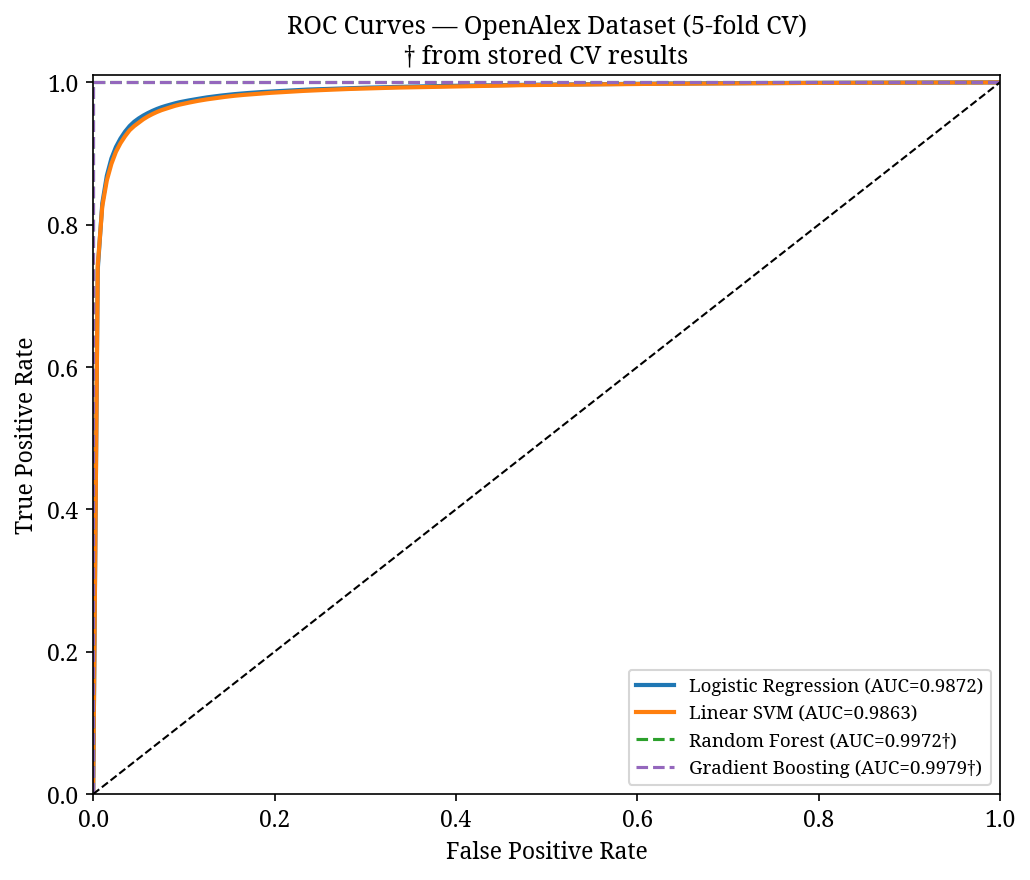
\includegraphics[width=0.75\textwidth]{../figures/oa/oa_fig4_roc_curves.png}
\caption{ROC curves for all models evaluated on the OpenAlex dataset.}
\label{fig:oa_roc}
\end{figure}

\begin{figure}[h!]
\centering
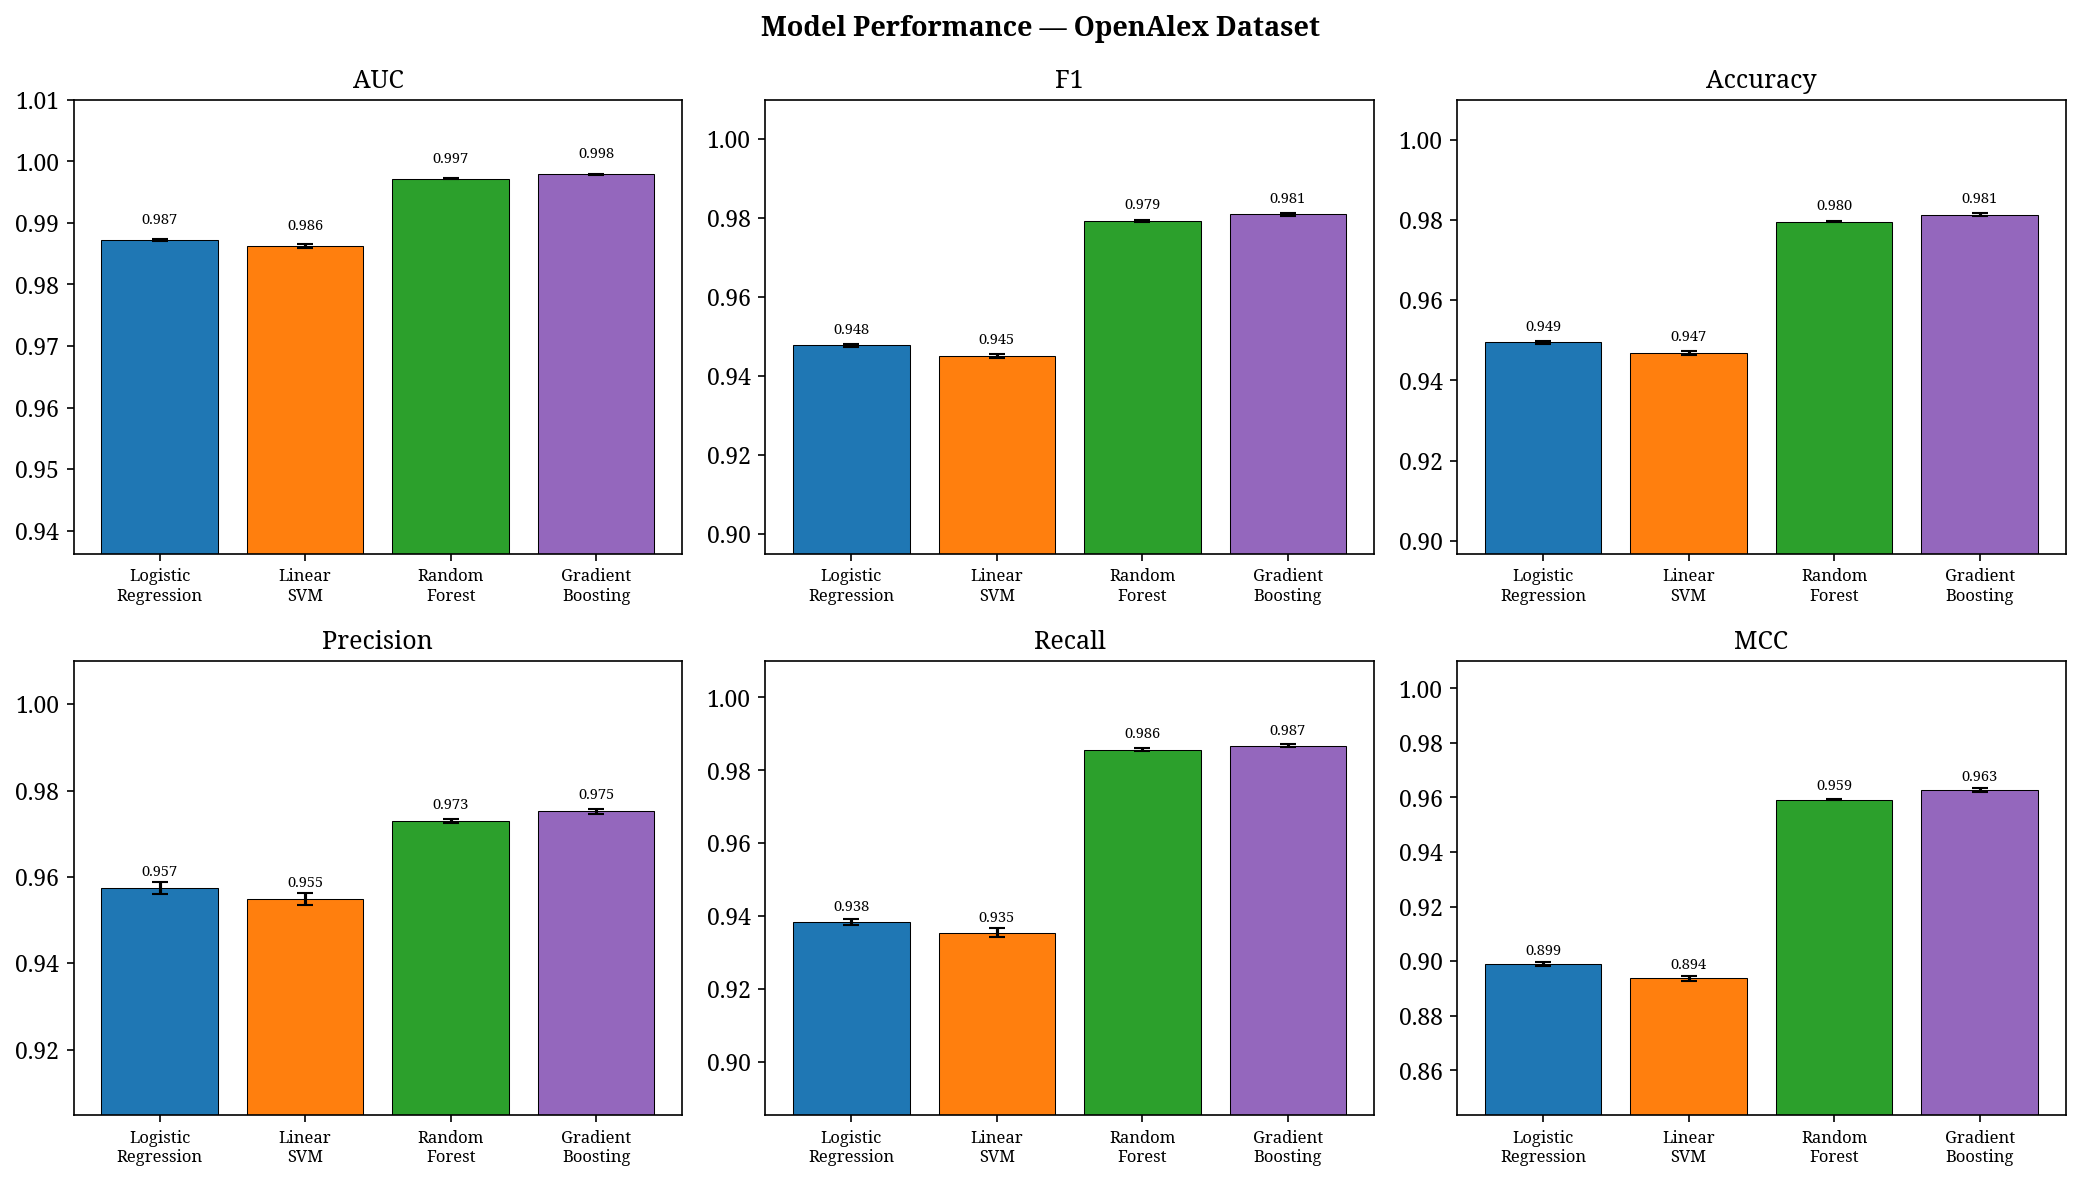
\includegraphics[width=0.75\textwidth]{../figures/oa/oa_fig5_model_comparison.png}
\caption{Model comparison across all performance metrics on the OpenAlex dataset.}
\label{fig:oa_compare}
\end{figure}

\subsection{Feature Importance and Explainability}

\subsubsection{SHAP Analysis}

SHAP analysis on the Gradient Boosting model for OpenAlex revealed a different feature hierarchy compared to Dimensions. Here, \textbf{activity\_citing} (mean absolute SHAP value 4.71) and \textbf{prestige\_cited} (4.50) were the top predictors, followed by \textbf{semantic\_similarity} (1.96). Temporal distance (0.80), common citers (0.64), and Jaccard reference similarity (0.62) contributed more modestly.

\begin{figure}[h!]
\centering
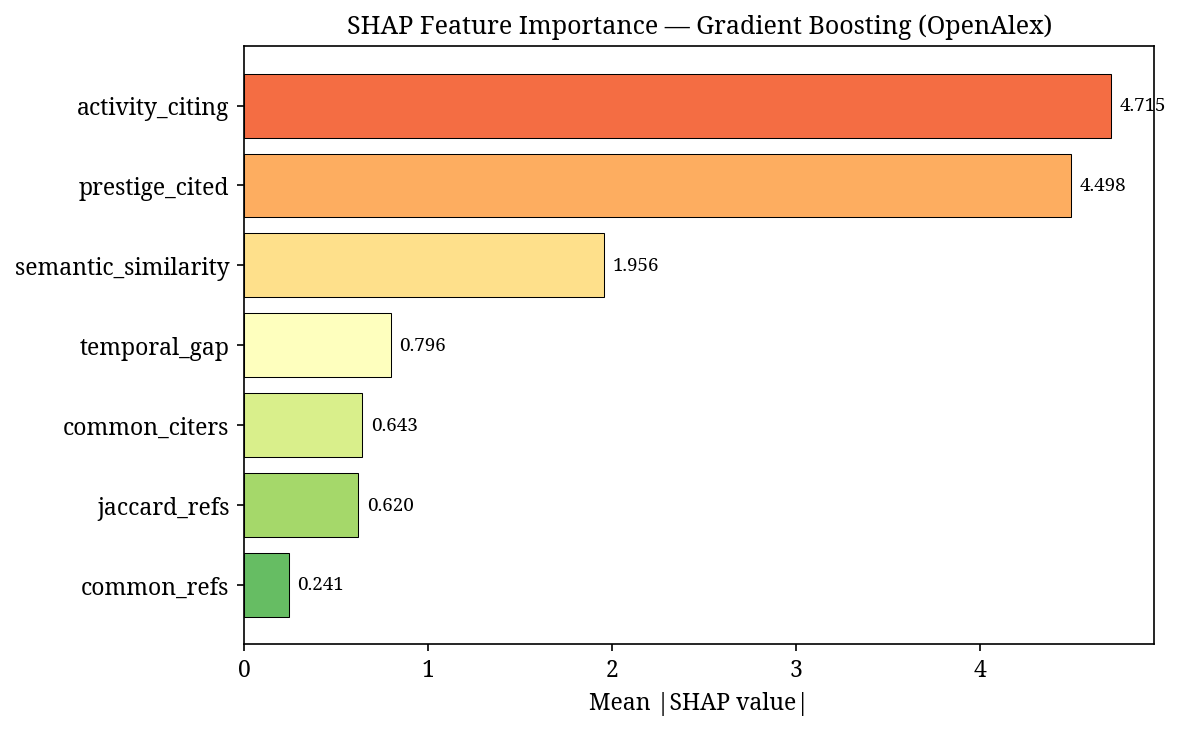
\includegraphics[width=0.75\textwidth]{../figures/oa/oa_fig6_shap.png}
\caption{Mean absolute SHAP values for the Gradient Boosting model on the OpenAlex dataset.}
\label{fig:oa_shap}
\end{figure}

The prominence of prestige features in the OpenAlex SHAP analysis, compared to the dominance of semantic similarity in Dimensions, suggests that the Matthew effect may be more pronounced in the OpenAlex LIS corpus. This could reflect differences in dataset construction, the broader time span covered, or the different feature set available. The larger temporal span of the OpenAlex dataset (1975--2024 vs. 1985--2023) may include more papers from periods when prestige effects were stronger, before the rise of open access and online search tools that democratized access to the literature.

\subsubsection{Ablation Study}

Table~\ref{tab:oa_ablation} presents the results of the leave-one-out ablation study on the OpenAlex dataset, using the Random Forest model.

\begin{table}[h!]
\centering
\caption{Feature Ablation Study (OpenAlex Dataset, Random Forest, Leave-One-Out)}
\label{tab:oa_ablation}
\begin{tabular}{lcc}
\toprule
\textbf{Feature Removed} & \textbf{ROC-AUC} & \textbf{Drop from All Features} \\
\midrule
None (all features) & 0.9972 & -- \\
prestige\_cited & 0.9847 & $-0.0125$ \\
activity\_citing & 0.9890 & $-0.0082$ \\
semantic\_similarity & 0.9914 & $-0.0058$ \\
temporal\_gap & 0.9960 & $-0.0012$ \\
common\_citers & 0.9970 & $-0.0002$ \\
jaccard\_refs & 0.9972 & $0.0000$ \\
common\_refs & 0.9972 & $0.0000$ \\
\bottomrule
\end{tabular}
\end{table}

The ablation results confirm the SHAP findings. Removing \texttt{prestige\_cited} causes the largest performance drop ($-0.0125$ AUC), followed by \texttt{activity\_citing} ($-0.0082$) and \texttt{semantic\_similarity} ($-0.0058$). The reference overlap features (Jaccard similarity, common references) contribute negligibly when all other features are present, suggesting that their information is largely captured by the prestige and semantic features.

The relatively small drop from removing semantic similarity ($-0.0058$) compared to the Dimensions result ($-0.1159$) is striking. This difference likely reflects the different feature sets: in Dimensions, semantic similarity is the only content-based feature, while in OpenAlex, the reference overlap features (common references, Jaccard similarity) provide complementary content-based signals. When semantic similarity is removed from the OpenAlex model, the reference overlap features partially compensate, limiting the performance drop.

%% ============================================================
\section{Comparative Analysis: Dimensions vs.\ OpenAlex}
\label{sec:comp}
%% ============================================================

\subsection{Overall Predictive Performance}

Both datasets yield models with exceptional predictive performance (ROC-AUC $> 0.99$), confirming that citation dynamics in LIS are highly predictable from historical network and semantic states, regardless of the data source. This robustness across two independent datasets, constructed using different methodologies and covering different time periods, substantially strengthens the validity of our conclusions.

\begin{figure}[h!]
\centering
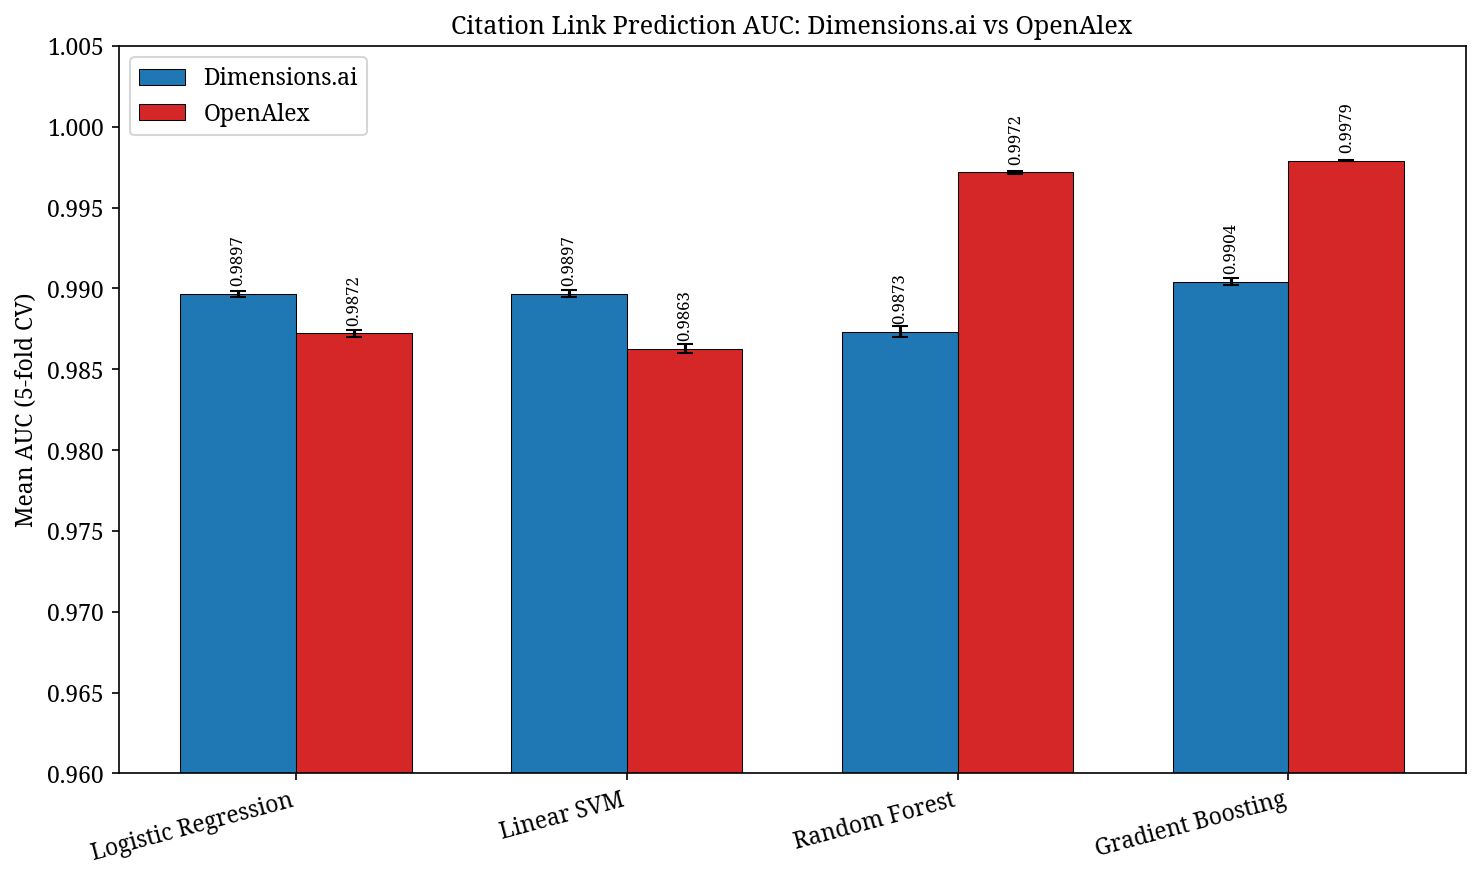
\includegraphics[width=0.75\textwidth]{../figures/comp_fig1_auc_comparison.png}
\caption{Comparison of best model ROC-AUC between Dimensions and OpenAlex datasets.}
\label{fig:comp_auc}
\end{figure}

Figure~\ref{fig:comp_auc} shows the AUC comparison between the two datasets. The OpenAlex Gradient Boosting model (AUC 0.9979) outperforms the Dimensions MLP (AUC 0.9906), though both are exceptional. The larger performance gap between linear and non-linear models in OpenAlex suggests that the OpenAlex feature set captures more complex, non-linear interactions.

\begin{figure}[h!]
\centering
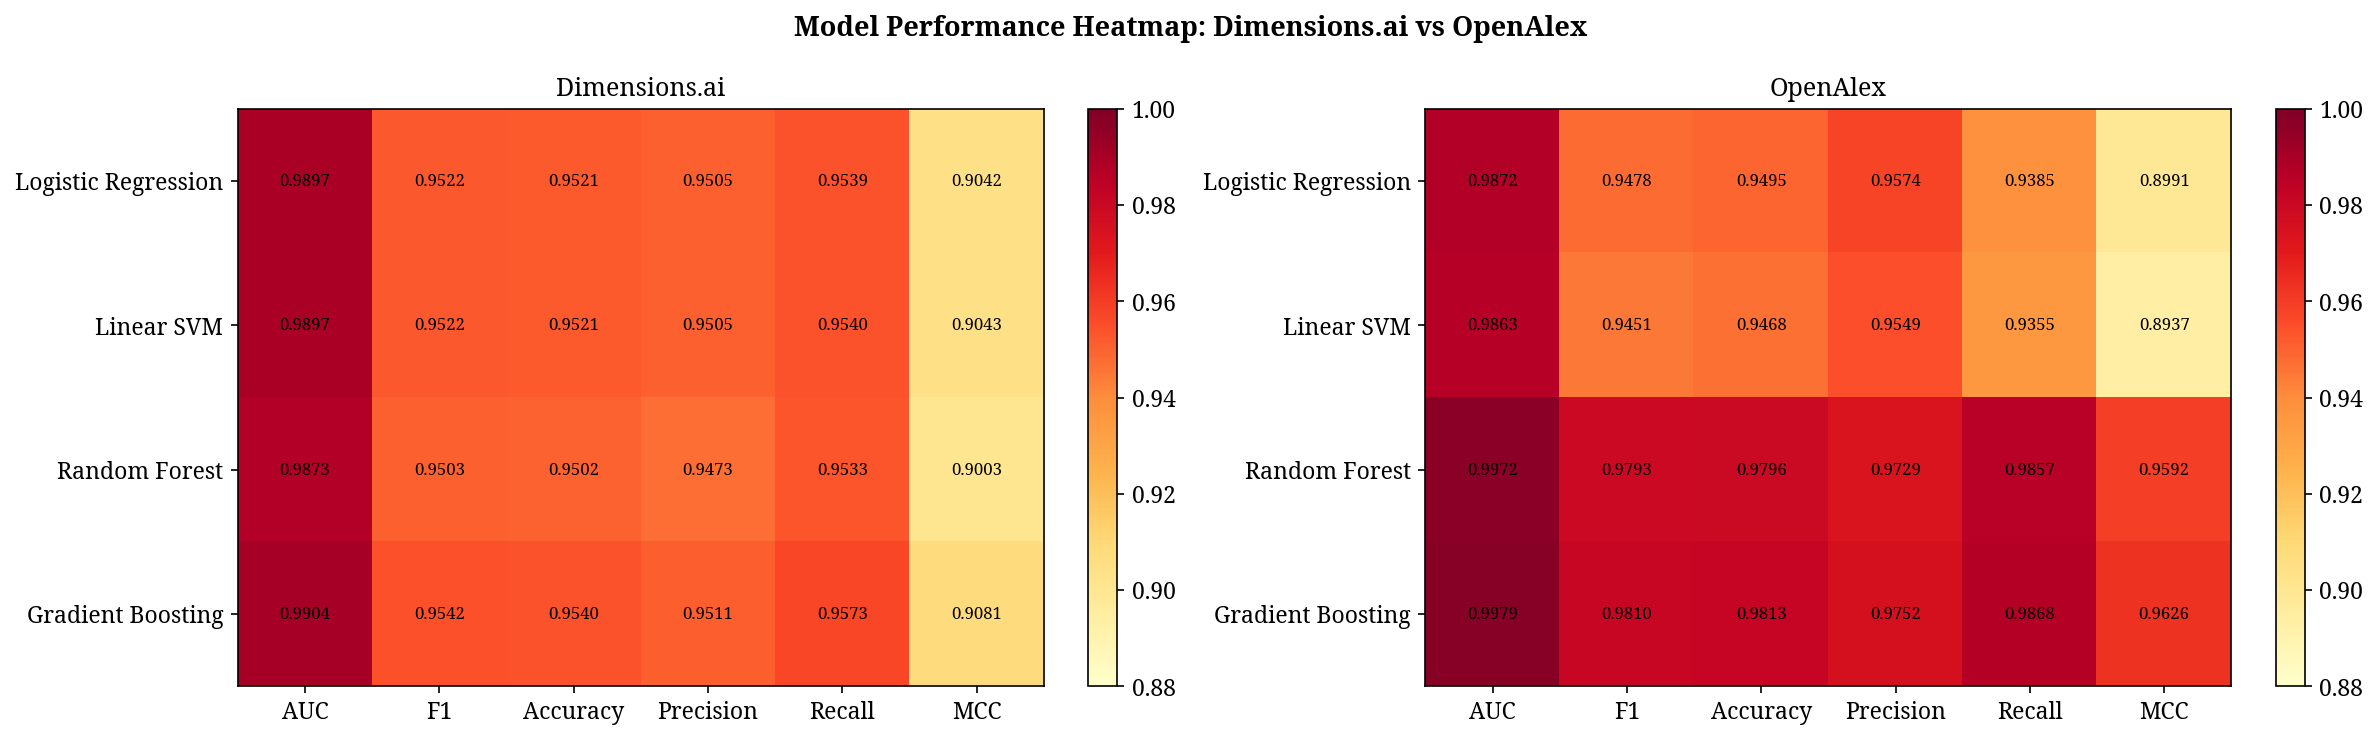
\includegraphics[width=0.75\textwidth]{../figures/comp_fig2_metrics_heatmap.png}
\caption{Full metrics comparison heatmap for both datasets.}
\label{fig:comp_metrics}
\end{figure}

Figure~\ref{fig:comp_metrics} shows the full metrics comparison heatmap. Across all six metrics, the OpenAlex ensemble models consistently outperform their Dimensions counterparts, while the linear models perform comparably across datasets. This pattern suggests that the OpenAlex feature set---particularly the reference overlap features---provides richer non-linear structure that ensemble methods can exploit.

\subsection{Feature Importance Hierarchy}

The most striking difference between the two datasets lies in the relative importance of features. In the Dimensions dataset, semantic similarity was overwhelmingly the dominant predictor (SHAP 0.305), with prestige of the cited paper a distant second (0.137). In the OpenAlex dataset, prestige metrics (activity\_citing: 4.71, prestige\_cited: 4.50) edged out semantic similarity (1.96) as the top predictors.

\begin{figure}[h!]
\centering
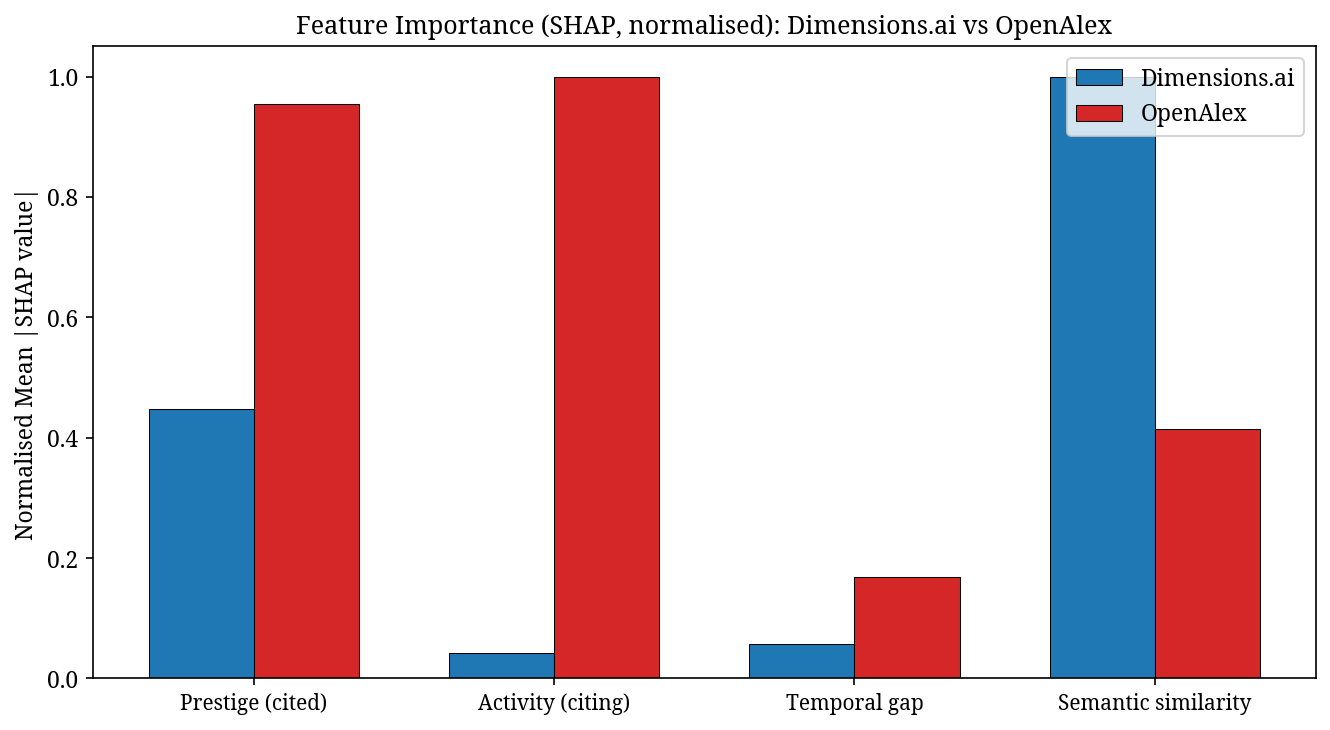
\includegraphics[width=0.75\textwidth]{../figures/comp_fig3_shap_comparison.png}
\caption{Normalized SHAP feature importance comparison between Dimensions and OpenAlex datasets.}
\label{fig:comp_shap}
\end{figure}

This discrepancy may reflect several factors. First, the Dimensions dataset includes co-authorship distance as a feature, which may partially absorb variance that would otherwise be attributed to prestige. Second, the OpenAlex dataset covers a longer time period (1975--2024 vs. 1985--2023), potentially including more papers from periods when prestige effects were stronger. Third, the specific topic coverage of the two datasets may differ, with different subfields of LIS exhibiting different citation dynamics.

Despite these differences, a consistent finding emerges: in both datasets, the \textit{combination} of semantic and prestige features is necessary to achieve the highest performance. Neither semantic similarity alone nor prestige alone is sufficient; it is the interaction between content relevance and established impact that drives citation decisions.

\subsection{Semantic Similarity Distributions}

Figure~\ref{fig:comp_sem} compares the distributions of semantic similarity for positive and negative pairs across the two datasets. Both datasets show a clear separation, with positive pairs exhibiting substantially higher semantic similarity than negative pairs. The mean semantic similarity for positive pairs is 0.5573 (Dimensions) and 0.5183 (OpenAlex), compared to 0.1624 and 0.2161 for negative pairs, respectively.

\begin{figure}[h!]
\centering
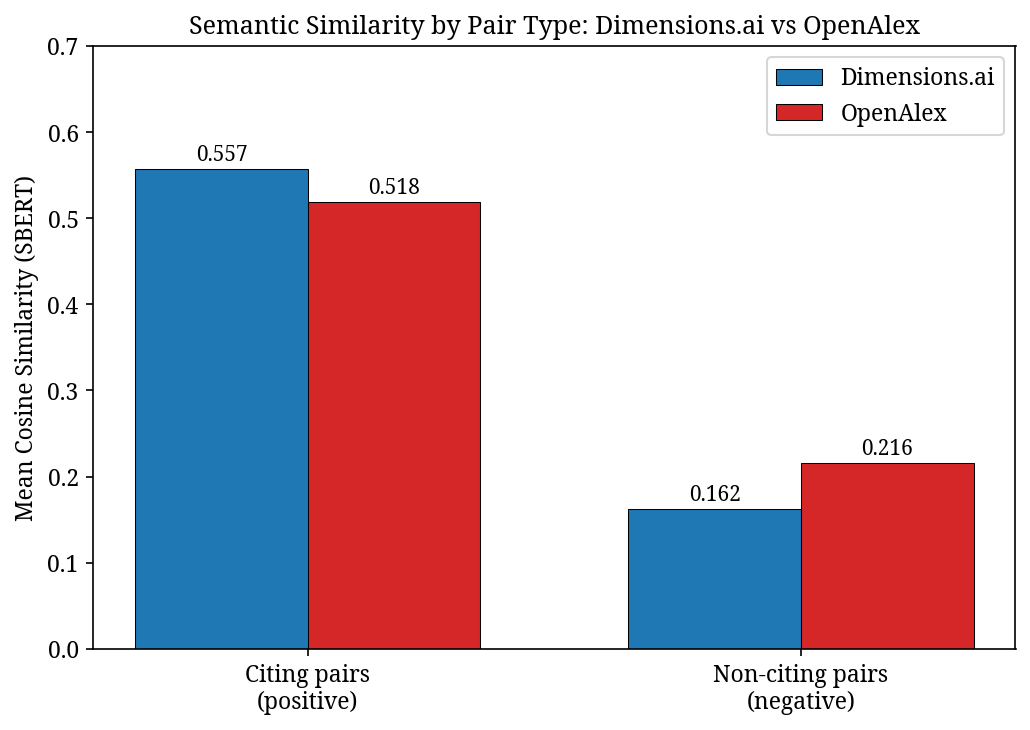
\includegraphics[width=0.75\textwidth]{../figures/comp_fig4_semantic_sim_comparison.png}
\caption{Semantic similarity distributions for cited and not-cited pairs across both datasets.}
\label{fig:comp_sem}
\end{figure}

The slightly higher mean similarity for positive pairs in Dimensions (0.5573 vs. 0.5183) and the slightly lower mean for negative pairs (0.1624 vs. 0.2161) suggest that the Dimensions dataset exhibits stronger semantic clustering of citation behavior. This could reflect the more targeted nature of the Dimensions query (using FoR codes and specific keywords) compared to the OpenAlex topic-based retrieval, which may include a broader range of papers with more diverse citation patterns.

\subsection{Summary of Cross-Dataset Findings}

Table~\ref{tab:crossdataset} summarizes the key findings across the two datasets.

\begin{table}[h!]
\centering
\caption{Summary of Cross-Dataset Findings}
\label{tab:crossdataset}
\begin{tabular}{lcc}
\toprule
\textbf{Characteristic} & \textbf{Dimensions} & \textbf{OpenAlex} \\
\midrule
Best model & MLP Neural Network & Gradient Boosting \\
Best AUC & 0.9906 & 0.9979 \\
Top feature (SHAP) & Semantic similarity & Activity (citing) \\
2nd feature (SHAP) & Prestige (cited) & Prestige (cited) \\
Linear vs. ensemble gap & Small ($\sim$0.001) & Large ($\sim$0.010) \\
Ablation: biggest drop & Semantic ($-0.116$) & Prestige ($-0.013$) \\
Mean sem. sim. (positive) & 0.5573 & 0.5183 \\
Mean sem. sim. (negative) & 0.1624 & 0.2161 \\
\bottomrule
\end{tabular}
\end{table}

%% ============================================================
\section{Discussion}
\label{sec:discussion}
%% ============================================================

\subsection{Theoretical Implications}

Our findings advance the theoretical understanding of citation dynamics in several important ways. First, the exceptional predictive performance of our models (ROC-AUC $> 0.99$) demonstrates that citation decisions are not random or idiosyncratic but follow systematic patterns that can be captured by a small set of well-engineered features. This finding supports the view of citation as a structured social and intellectual process, governed by regularities that transcend individual researcher preferences.

Second, the dominance of semantic similarity in the Dimensions dataset and prestige in the OpenAlex dataset highlights the context-dependence of citation dynamics. The relative importance of content relevance versus established impact may vary across datasets, time periods, and subfields. This finding calls for caution in generalizing from single-dataset studies and underscores the value of multi-dataset analyses like the present one.

Third, the clear superiority of ensemble methods over linear models in the OpenAlex dataset provides strong evidence for complex, non-additive interactions between predictors. A paper with moderate prestige might still be cited if its semantic relevance is exceptionally high---a non-linear dynamic that tree-based models capture effectively. This finding aligns with the broader literature on the complexity of citation dynamics \citep{fortunato2018science, zeng2017science}.

Fourth, the ablation studies confirm that the combination of semantic and structural features is essential for optimal performance. Neither feature class alone achieves the performance of the full model, and the marginal contribution of each feature class varies across datasets. This finding supports a multi-dimensional view of citation behavior, in which content relevance, social proximity, and prestige jointly shape citation decisions.

\subsection{The Matthew Effect and Its Limits}

Our results provide nuanced evidence regarding the Matthew effect in LIS citation dynamics. On one hand, prestige features (particularly the citation count of the cited paper) are consistently among the top predictors in both datasets, confirming that highly cited papers attract disproportionate future citations. On the other hand, the dominance of semantic similarity in the Dimensions dataset suggests that the Matthew effect is not the primary driver of citation behavior in this corpus.

This finding is consistent with the ``fitness'' model of citation dynamics \citep{bianco2008fitness, wang2013quantifying}, which posits that the long-term impact of a paper is determined by a combination of its intrinsic quality (captured here by semantic relevance) and its initial prestige. Papers that are both highly relevant and highly cited are most likely to be cited in the future, while papers that are relevant but not yet well-known may be systematically undervalued by citation metrics.

The relatively modest contribution of co-authorship distance in the Dimensions dataset (SHAP $\approx 0.022$) suggests that social proximity plays a secondary role in LIS citation dynamics, at least when semantic and prestige features are also available. This finding contrasts with the strong social proximity effects reported in some other disciplines \citep{newman2004coauthorship, martin2013coauthorship} and may reflect the relatively small and interconnected nature of the LIS research community.

\subsection{Methodological Contributions}

Our study makes several methodological contributions to the citation prediction literature. The strict temporal causality framework we propose addresses a fundamental flaw in many existing studies and provides a template for future work. By computing all features using only information available at the time of the citation decision, we ensure that our models reflect genuine predictive relationships rather than post-hoc correlations.

The use of SBERT for semantic embedding represents a significant advance over earlier approaches based on TF-IDF or LDA. SBERT captures subtle semantic relationships that are invisible to bag-of-words methods, enabling more accurate measurement of content similarity. The high SHAP values for semantic similarity in both datasets confirm the value of this approach.

The SHAP analysis and ablation studies provide interpretable insights that go beyond simple feature importance rankings. By quantifying the marginal contribution of each feature class, we can identify which aspects of citation behavior are most amenable to prediction and which remain unexplained by our current feature set.

\subsection{Implications for Research Evaluation}

Our findings have important implications for research evaluation practice. The high predictability of citations from semantic and prestige features suggests that citation-based metrics may be capturing genuine intellectual influence rather than mere social network effects. However, the strong effect of prestige (the Matthew effect) also implies that citation metrics may systematically undervalue the contributions of less-established researchers, even when their work is semantically relevant to ongoing research streams.

These findings support the growing movement toward more nuanced research evaluation frameworks that consider multiple dimensions of impact, including semantic relevance, social network position, and temporal dynamics. The framework developed in this study could be used to construct ``expected citation'' baselines that account for the predictable components of citation behavior, enabling fairer comparisons of research impact across researchers with different career stages and network positions.

\subsection{Limitations}

This study has several limitations that should be acknowledged. First, our analysis is restricted to a single field (Library and Information Science). The relative importance of social, semantic, and prestige factors may vary substantially across other disciplines, particularly between the hard sciences, social sciences, and humanities. Future work should extend this framework to other fields to test the generalizability of our findings.

Second, while we strictly enforced temporal causality in feature construction, observational data cannot definitively establish causal mechanisms. The correlations we observe between features and citation outcomes may reflect confounding factors not captured in our feature set. For example, the apparent effect of semantic similarity may partly reflect the tendency for papers in the same subfield to both cite each other and to use similar terminology.

Third, the OpenAlex dataset has relatively low coverage of reference lists (29.8\%), which may introduce selection bias in the construction of citation pairs. Papers with available reference lists may differ systematically from those without, potentially affecting the generalizability of our findings.

Fourth, the exclusion of k-NN and Neural Network models from the OpenAlex analysis due to memory constraints limits the direct comparability of results across datasets. Future work with more computational resources should evaluate all six models on both datasets.

%% ============================================================
\section{Conclusion}
\label{sec:conclusion}
%% ============================================================

This paper demonstrates that machine learning approaches, when constrained by strict temporal causality, offer a powerful framework for understanding and predicting citation dynamics in Library and Information Science. By integrating network science (co-authorship distance and reference overlap), natural language processing (SBERT semantic embeddings), and advanced machine learning (ensemble methods and neural networks), we constructed predictive models that achieve exceptional accuracy (ROC-AUC $> 0.99$) across two independent bibliographic datasets.

Our SHAP analysis and ablation studies reveal that citation dynamics are driven by a combination of content relevance (semantic similarity), established impact (prestige), and social proximity, with the relative importance of these factors varying across datasets. The combination of all feature classes is necessary for optimal performance, confirming the multi-dimensional nature of citation behavior.

The comparative analysis of Dimensions and OpenAlex datasets demonstrates the robustness of our framework across data sources while also highlighting dataset-specific differences that call for further investigation. Future work should extend this framework to other disciplines, investigate the temporal evolution of feature importance, and develop interpretable models that can provide actionable insights for researchers and research evaluators.

The integration of machine learning with traditional bibliometric and network science approaches offers a powerful new lens through which to examine the mechanisms that drive scientific impact and the structure of the scientific enterprise itself. By establishing a rigorous, temporally-aware methodological standard, this study provides a foundation for future predictive modeling in bibliometrics.

\newpage
\bibliographystyle{plainnat}
\bibliography{references}

\end{document}
